\documentclass{jdrp}

\bibliography{references} 

\newcommand*{\crg}{{\aurebesh\Large \$}} % Symbol for Galactic Credits

\hypersetup{  
  pdfinfo={  
    Title={SWR - Dos au Muur},
    Subject={Star Wars Redemption, campagne Dos au Muur, version 1.0.1},
    Author={Marthym},
    Keywords={star,wars,savage,worlds,jdra,jdrp,scenario,muur,talisman},  
    Copyright={Do What The Fuck You Want To Public License}
  }  
} 

\begin{document}

	\begin{titlepage}

	\begin{center}
		\hspace*{\vfill}
		\noindent\Huge\jedifont{Star Wars Redemption}\\ 
		\noindent\fontsize{50}{70}\jedifont{\$}
		\noindent\fontsize{50}{70}\jedifont{\#}\\
		\noindent\fontsize{50}{60}\jedifont{Dos au Muur}
		\hspace*{\vfill}
	\end{center}

	\noindent\makebox[\textwidth]{
		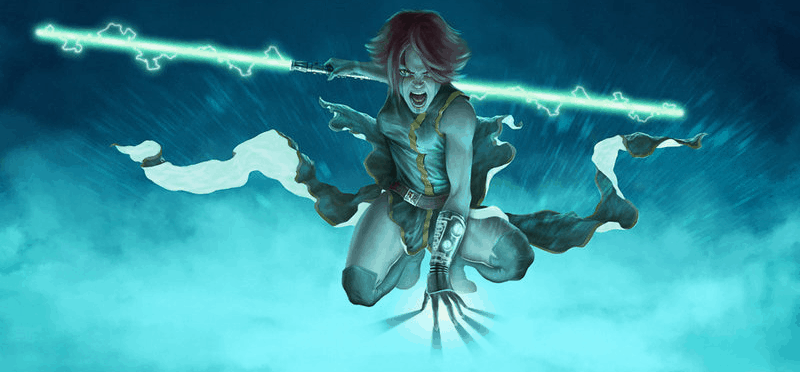
\includegraphics[width=\paperwidth]{swr-class/_img/cover-bg.jpg}}
	\begin{tikzpicture}[overlay]
		\node[minimum width=180pt,minimum height=180pt, rotate=30] at (15,11){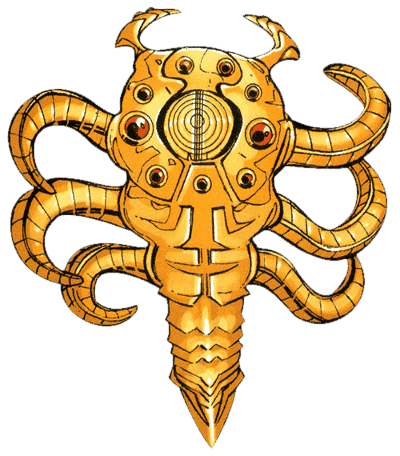
\includegraphics[width=180pt]{_img/talisman.png}};
	\end{tikzpicture}}
	\end{titlepage}

	\onecolumn
	\section{contexte de campagne}
	
	\begin{wrapfigure}{R}{180pt}
		\centering
		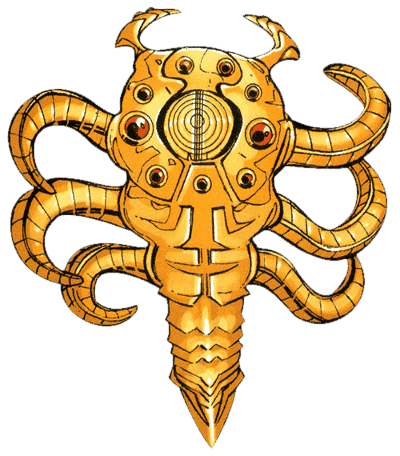
\includegraphics[width=180pt]{_img/talisman.png}
		\caption{\label{fig:talisman-de-muur}Talisman de Muur}
		\vspace{1\baselineskip}
		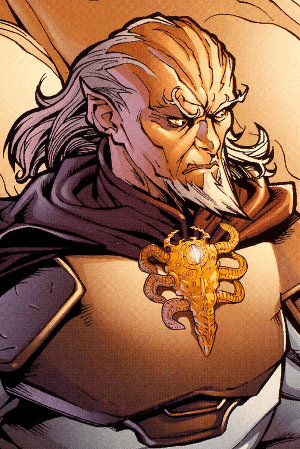
\includegraphics[width=180pt]{_img/pnjs/karness-muur.jpg}
		\caption{\label{fig:karness-muur}Karness Muur}
	\end{wrapfigure}
	
	Cette campagne est écrite initialement pour \citetitle{jdrp-starwars} mais un scénar reste un scénar et il est jouable dans n’importe quel univers de Star Wars.

	L’idée était de faire une campagne d’introduction avec des personnages partant de rien. Les joueurs commencent Novice et n’ont pas besoin d’historique complexe et élaboré (bien que cela ne soit pas interdit bien sûr). De cette façon, les personnages devraient être assez vite fait. Et elle est adaptable aussi bien avec des joueurs orienté Alliance Rebelle que Empire. Dans les deux cas, l’objectif sera le même mais les dessains changeront.

	La campagne se déroule dans les premières années de l’avènement de l’Empire, au MJ de voir s’il veut préciser.

	La trame de la campagne se base sur un très ancien artefact Sith, le \citetitle{talisman-de-muur}. Un artefact créé par Karness Muur, un Sith se servant de la Force pour prolonger sa vie. L’artefact contient l’âme de Muur, celui qui le porte est possédé par Karness et peut contrôler les Rakghoules.


	On trouve beaucoup d’informations sur cet artefact sur HoloNet et je me suis grandement inspiré de ces informations pour cette campagne en faisant vivre à mes héros les aventures de divers protagonistes ayant croisé le Talisman\ldots

    \subsubsection{Note sur le PDF}

    Ce PDF contient deux calques. La couleur de fond des pages peu être masqué pour une meilleure qualité d’impression.


	\twocolumn

	\section{Sauvetage du Pelican}

Voici un premier scénario pour la campagne \textbf{Dos au Muur}. 

\subsection{La rencontre}
Nos héros ne se connaissent pas encore. Ils ont répondu à un contrat proposé par \emph{Industrial Automaton} pour une mission de récupération.

\begin{paperbox}{Notes sur les personnages}
	Je n’aime pas brider les joueurs sur leur choix de concept de personnage. Mais des fois l’imagination des joueurs dépasse légèrement le cadre de nos scénarios. Alors voici quelques exemples de concepts et comment il est possible de les intégrer :
	\begin{rebelist}
		\item Des \textbf{mercenaires} et chasseurs de primes, qui du coup s’intègrent très bien dans le scénario
		\item Un \textbf{mécano} touche à tout, qui était envoyé par IA pour sa connaissance du vaisseau ou du modèle R4
		\item Un \textbf{noble}, qui en tant qu’investisseur voulait savoir ou passe son argent (et IA qui voulant s’en débarrasser a accepté avec plaisir)
	\end{rebelist}
\end{paperbox}

Ils ont rendez-vous sur l’avant-poste commercial de l’anneau de Kafrene au Starlord Café. \'A leur arrivée, ils sont conviés dans une arrière salle ou les attend \nameref{sec:vyna-anen} un Sluissi, le représentant de IA. En plus du groupe de nos héros, deux autres personnes ont répondu au contrat, un Abyssin et un Rodien.

\begin{quotebox}
	Messieurs bonjour, je représente Indrustrial Automaton.
	Comme vous avez peu le voir sur le contrat auquel vous avez répondu, nous cherchons à rassembler une équipe pour récupérer l’un de nos prototypes de droïde Type R perdu sur un Croiseur dont nous n’avons plus de nouvelle.
	Le \textbf{Pelican IA-1701} n’a plus donné signe de vie depuis 10h et 33mn maintenant. Il avait à son bord le seul prototype de notre dernier Type R. Il est vital pour nous de récupérer ce prototype intact.

	Si vous acceptez la mission, une navette droïde vous conduira directement à la dernière position connue du Pelican. Cette mission doit resté confidentielle, nous ne tenons pas à ce que le public sache qu’Industrial Automaton perde ses vaisseaux !
	En cas de succès la somme convenue sera virée directement sur vos comptes respectifs. Dans le cas contraire vous serez mort ou en passe de l’être.

	Y a-t’il des questions ?

	\ldots

	Bien, la navette décollera de l’astroport, quai N°5 dans une heure, elle n’attendra personne.
\end{quotebox}

Voilà qui donne le ton et la direction du scénario. Les héros disposent donc d’une heure, s’ils le souhaitent pour faire quelques emplettes puis direction la navette. Si des joueurs demandent à prendre leur propre vaisseau, cela est impossible, l'emplacement du vaisseau doit rester confidentiel.

\subsection{Pelican Bay}
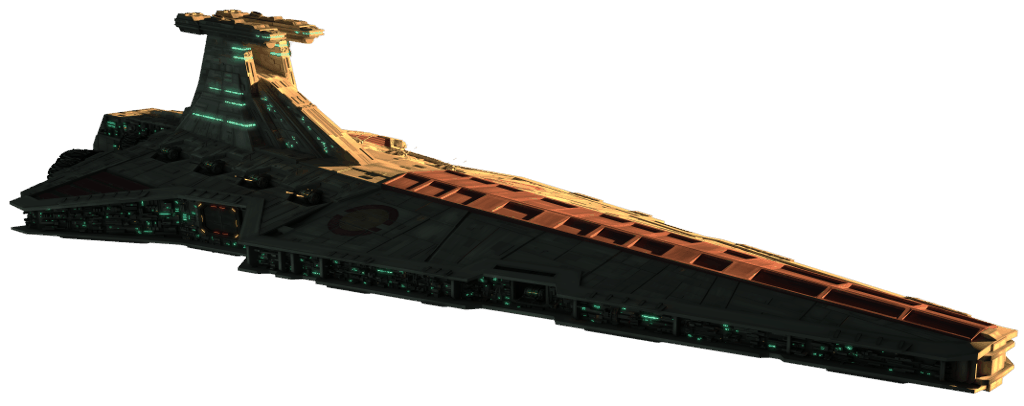
\includegraphics[width=\linewidth]{_img/venator.png}
\'A la sortie d’hyperespace, les héros trouvent croiseur de classe Venator en bon état mais à la dérive. La navette tente une procédure d’appontage mais le système de guidage ne semble pas fonctionner, le droïde aux commandes de la navette ne cesse de répéter :
\begin{quotebox}
	Erreur trop bas trop bas !\\
	Erreur trop bas trop bas !\\
	Erreur trop bas trop bas !\\
	Erreur trop bas trop bas !\\
	Erreur trop bas trop bas !\ldots
\end{quotebox}

Et la navette s’échoue lamentablement dans le hangar. Comme de par hasard, et pour bien appuyer sur la gravité de la situation, l’Abyssin et le Rodien sont mort pendant le crash et le droïde pilote est dans un sale état. Il ne pourra donner aucune information.

Une fois à bord du Pelican, une alarme est en cours et une voie pré-enregistrée se fait entendre à intervalles réguliers :

\begin{quotebox}
	Alerte trajectoire, le vaisseau se dirige actuellement vers une étoile, point de non-retour dans 2h53mn ! 
	Voyez modifier la trajectoire du vaisseau !\\ 
	\ldots
\end{quotebox}

\'A l’intérieur du vaisseau c’est la désolation, des cadavres partout, du sang sur les murs, des traces de griffures sur les murs. L’éclairage est partiellement en panne les néons scintillent, des débris entravent la marche des héros. Leur champ de vision est réduit à cause des conditions à bord. Malgré tout ça, les systèmes de survie et la gravité artificielle fonctionnent.\\

Le bruit du crash de la navette a attiré la population locale, à savoir les Rakghouls~\ref{sec:rakghoul} (p. \pageref{sec:rakghoul}). Lancer 1d4 pour savoir combien se pointent. Si vous n’avez que 2 ou trois héros sous la main, ajustez avec 1d4-1.

\noindent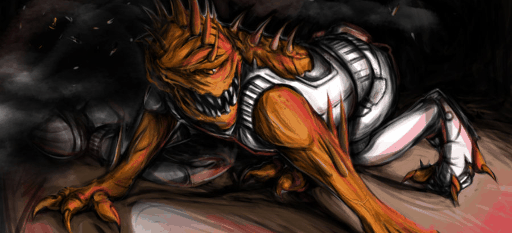
\includegraphics[width=\linewidth]{_img/bestiary/rakghoul.png}

Le but des héros devrait maintenant être double, trouver le fameux prototype mais aussi trouver un moyen de sauver leur peau. 

\subsection{Exploration}
\emph{Numérotez les pièces de votre vaisseau et lancez un dé pour savoir dans quelle pièce se trouve le droïde.}\\

Une fois la première vague de Rakghouls balayé, nos héros se retrouvent dans le hangar, la porte de se dernier est ouverte.

Un jet de Recherche (-2 pour l’obscurité) réussi permet de trouver un kit de survie avec un Medipac, une lampe torche et des rations de survie.

Pas loin de la porte du hangar se trouve un terminal dont l’écran clignote en rouge au rythme de l’alarme. Les héros peuvent tenter des jets de Piratage pour les actions suivantes :
\begin{rebelist}
	\item Stopper l’alarme. 
	\item Obtenir un plan du vaisseau. En cas de succès, le plan s’affiche mais le terminal rend l’âme au bout de quelques secondes et le plan s’efface. En cas de relance le plan reste affiché et le terminal est utilisable.
	\item Obtenir l’inventaire des navettes présente dans les hangars du vaisseau. Un succès leur apprend qu’il y en a une dans le hangar du niveau inférieur. Une Relance leur apprend que la navette est dans le hangar 4-2.
\end{rebelist}
Dans tous les cas, un échec critique fait disjoncter le terminal définitivement.

Les héros avancent donc dans les couloirs du Pelican à la recherche du droïde et d’un moyen de dévier le vaisseau. Faites faire un jet de Discrétion de temps à autre. En cas d’échec, 2 Rakghouls se pointent (plus si vous voyez que vos héros s’en tire trop facilement).

Au fur et mesure que les aventuriers avancent, utilisez les tuiles pour découvrir la carte du vaisseau.

\subsubsection{Le Droïde}
Quand les héros arrivent dans la salle où se trouve le droïde (\nameref{sec:r4-3d}), ce dernier les menace avec un arc électrique, rien de bien méchant mais les héros doivent le rassurer et Négocier (jet de Persuasion) avec le droïde ou le Pirater (jet de Piratage opposé à l’Intellect). Dans les deux cas, avec un succès, le droïde les aide, leur montre le journal de bord. Avec une Relance, le droïde devient un acolyte du héros qui a fait l’action. En cas d’échec le droïde refuse de les aider il se désactive. En cas d’échec critique, le droïde s’en prend à eux.

Si le droïde se désactive, un héros peut tenter de lui retirer la mémoire pour récupérer les infos avec un jet de Réparation. 

\subsubsection{Les Quartiers}
Il s’agit des quartiers de l’équipage. Pas grand-chose à y trouver, des vêtements, des effets personnels. On y trouve des terminaux qui peuvent être Piraté pour le plan du vaisseau ou pour d’autres informations. Avec un succès, ils se connectent et ont accès au contenu du PC. La carte s’ils la cherchent, sinon rien de fou, des photos, des vidéos et des films X.

\subsubsection{Les Laboratoires}
La porte du premier labo que les héros visitent est verrouillé. un jet de Piratage la déverrouille. Si le droïde est avec eux et les aide, il peut ouvrir toutes les portes. Les aventuriers trouvent dans ce labo le corps du rakghoul et un terminal. Un Piratage (malus -2, c’est un terminal sécurisé) leur donne les informations sur l’autopsie (cf. Le \nameref{sec:pelican-jdb} p. \pageref{sec:pelican-jdb}), pas plus sur les circonstances.

Dans les autres labos, un jet de recherche donne un Medipac supplémentaire.

\subsubsection{L’Armurerie}
Dans cette pièce se trouvent des cellules énergétiques pour les armes et des armes mais enfermées dans des casiers. Un coup de blaster ouvre les casiers. On trouve alors 
\begin{rebelist}
	\item 5x Blaster semi-automatique \emph{(2d8 (3))}
	\item 1x Lance-Grenades \emph{(2d10 (1))}
	\item 5x Grenade \emph{(3d6)}
\end{rebelist}

\subsubsection{La Passerelle}
La pièce est verrouillée et ne peut être ouverte avec un Piratage. Seul le droïde peut l’ouvrir. Si le droïde disparaît ou s’éteint, la salle s’ouvre. Les héros en entrant dans la pièce trouvent le corps décomposé du commandant. En recherchant dans les poches du commandant, ils trouvent un document marqué "Protocole d’Urgence" expliquant la marche à suivre en cas de problème (cf. Le \nameref{sec:pelican-jdb} p. \pageref{sec:pelican-jdb}). Le papier contient aussi les codes d’accès au terminal.

Les héros peuvent donc accéder au \nameref{sec:pelican-jdb} avec toutes les infos. Si cela n’est déjà connu, ils savent qu’un vaisseau en état les attend dans le hangar 4-2 et il est possible d’en ouvrir la porte depuis ce terminal. S’ils sont malins, il est possible de voir ce qui les attend dans le hangar via des caméras de surveillance. Ils peuvent aussi déclencher l’autodestruction.

\begin{paperbox}{Objectifs}
Les joueurs doivent d’une manière ou d’une autre apprendre l’histoire des rakghouls et du Talisman. Donc soit par le droïde, soit par la passerelle. Une fois qu’une des deux étapes est passée, l’autre n’est pas obligatoire. Donc peu importe qu’ils déglinguent le droïde ou non.
\end{paperbox}

\subsection{Le hangar 4-2}

\noindent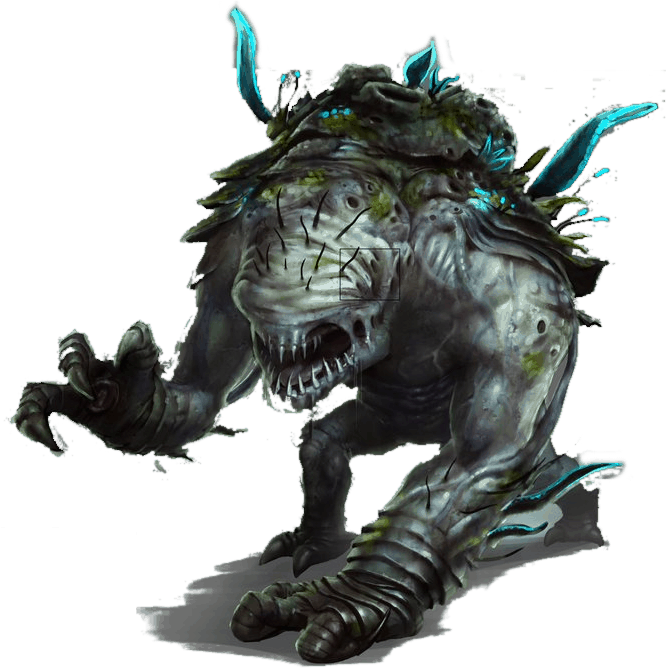
\includegraphics[width=\linewidth]{_img/bestiary/rakghoul-amblyope.png}

Situé au pont inférieur, deuxième hangar. C’est l’étape finale et le boss de fin du scénario.

Le droïde ou un passage au poste de commande déverrouille la porte du hangar. \'A l’intérieur c’est une autre histoire, une créature de 2m de haut manifestement un rakghoul aux stéroïdes, un rakghoul Amblyope~\ref{sec:rakghoul-amblyope} p. \pageref{sec:rakghoul-amblyope}).

Selon vos héros et leur état, accompagnez le joker avec quelques rakghouls en extra. Les héros avec Sens de Force ressentent une forte présence du côté obscur autour de la créature.\\

Une fois le combat terminé, il ne leur reste plus qu’à prendre le vaisseau (Cargo léger YZ-775, le \nameref{sec:nimbus}). Ouf, les clefs sont sur le contact. L’armement du vaisseau est endommagé et ne fonctionne pas mais le reste est intact.

\subsection{To be continue\ldots}
Une fois en vol, vos héros reçoivent une communication d’origine inconnue, le visage d’une femme apparaît

\begin{quotebox}
	Tinon \emph{(prononcer Taïnon)} c’est toi ? Que se passe t’il ou va tu ?
\end{quotebox}

Rideau, suite au prochain épisode\ldots

\subsection{Progression}
A titre indicatif car c’est a vous de voir ce que vos héros méritent.

\begin{rebelist}
	\item \textbf{1xp} Si vos héros ont R4-3D avec eux à la fin du scénar.
	\item \textbf{1xp} Pour avoir tué le \nameref{sec:rakghoul-amblyope}.
	\item \textbf{1xp} Pour être sortie du vaisseau en vie.
\end{rebelist}
Pas plus de 3xp, le scénar n’est pas assez long pour mériter plus.

\clearpage
\subsection{Pelican (iA-1701)} \label{sec:pelican}

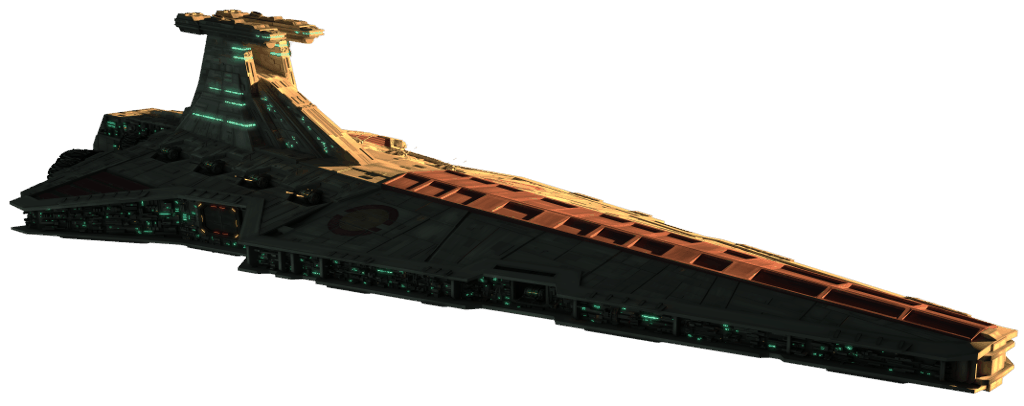
\includegraphics[width=\textwidth]{_img/venator.png}
\vspace{-4\baselineskip}

Quelques informations sur le Pelican. Il s’agit d’un croiseur de classe \textbf{Venator}. 1~137~m de long, 7400 hommes d’équipage, capable d’hyper-propulsion.

Le Pelican appartient à Industrial Automaton qui s’en sert comme vaisseau scientifique ultra-sécurisé. Ils y hébergent des projets top secret et aux limites de la loi.

\subsubsection{Journal de bord}
\label{sec:pelican-jdb}
En relation étroite avec l’Empire, Industrial Automation envoie le Pelican à la recherche d’un ancien artefact Sith, le Talisman de Muur. Le Pelican a fini par trouver une trace du Talisman sur \href{http://fr.starwars.wikia.com/wiki/Taris}{Taris}. En fouillant les bas fonds de la planète, l’équipe de chercheurs trouve les vestiges d'un ancien temple Sith. Malheureusement ce dernier est infesté de Rakghouls. L’unité de sécurité qui accompagne les chercheurs parvient à se débarrasser des quelques créatures mais plusieurs hommes sont blessés pendant le combat. Dans les ruines du temple le Talisman n’est plus là, mais des indices tendent à penser qu’il a été transporté il y a très longtemps vers une planète éloignée mais les scientifiques n’ont pas eu le temps d’en apprendre plus. Ils décident alors de ramener les corps des Rakghouls à bord du Pelican et de retourner sur Gaulus, une planète rocailleuse aux confins de la bordure extérieure.

En chemin vers Gaulus les scientifiques étudient le corps du Rakghoul et apprennent qu’il s’agit d’une maladie qui semble artificielle. La maladie se transmet par griffure ou morsure. Cette maladie est étroitement liée au côté Obscur de la Force et il semble que les personnes sensibles à la force ne puissent être contaminées. Cependant le Rakghoul étudié a l’air d’être contaminé par une forme très basique du virus, certainement une exposition prolongée à l’artefact.

Après une semaine de voyage, les problèmes ont commencé. Les soldats blessés lors de la rixe contre les Rakghouls sur Taris commencent à se transformer en Rakghouls à leur tour et s’en prennent aux membres de l’équipage. C’est une boucherie sans nom ! Voyant cela, le commandant du Pelican (\emph{Tycho Obrin}) déclenche le protocole d’urgence consistant à enregistrer le journal de bord sur un droïde Type R et tente de bloquer le cap du vaisseau sur l’étoile la plus proche. Mais la propulsion est endommagée et bien que le cap du vaisseau soit bloqué, ce dernier se contente de dériver.

\vspace{10\baselineskip}
\subsubsection{Industrial Automaton}
N’ayant plus de nouvelle du Pelican depuis son départ de Taris, IA part à sa recherche. Ils le retrouvent et envoient une équipe à son bord, mais là encore, plus aucune nouvelles. C’est alors qu’IA décide d’envoyer des mercenaires. Si le commandant a respecté le protocole, il suffira que les mercenaires ramènent le droïde\ldots

\onecolumn
\subsubsection{Plan du vaisseau}

\begin{figure}[!h]
	\centering
	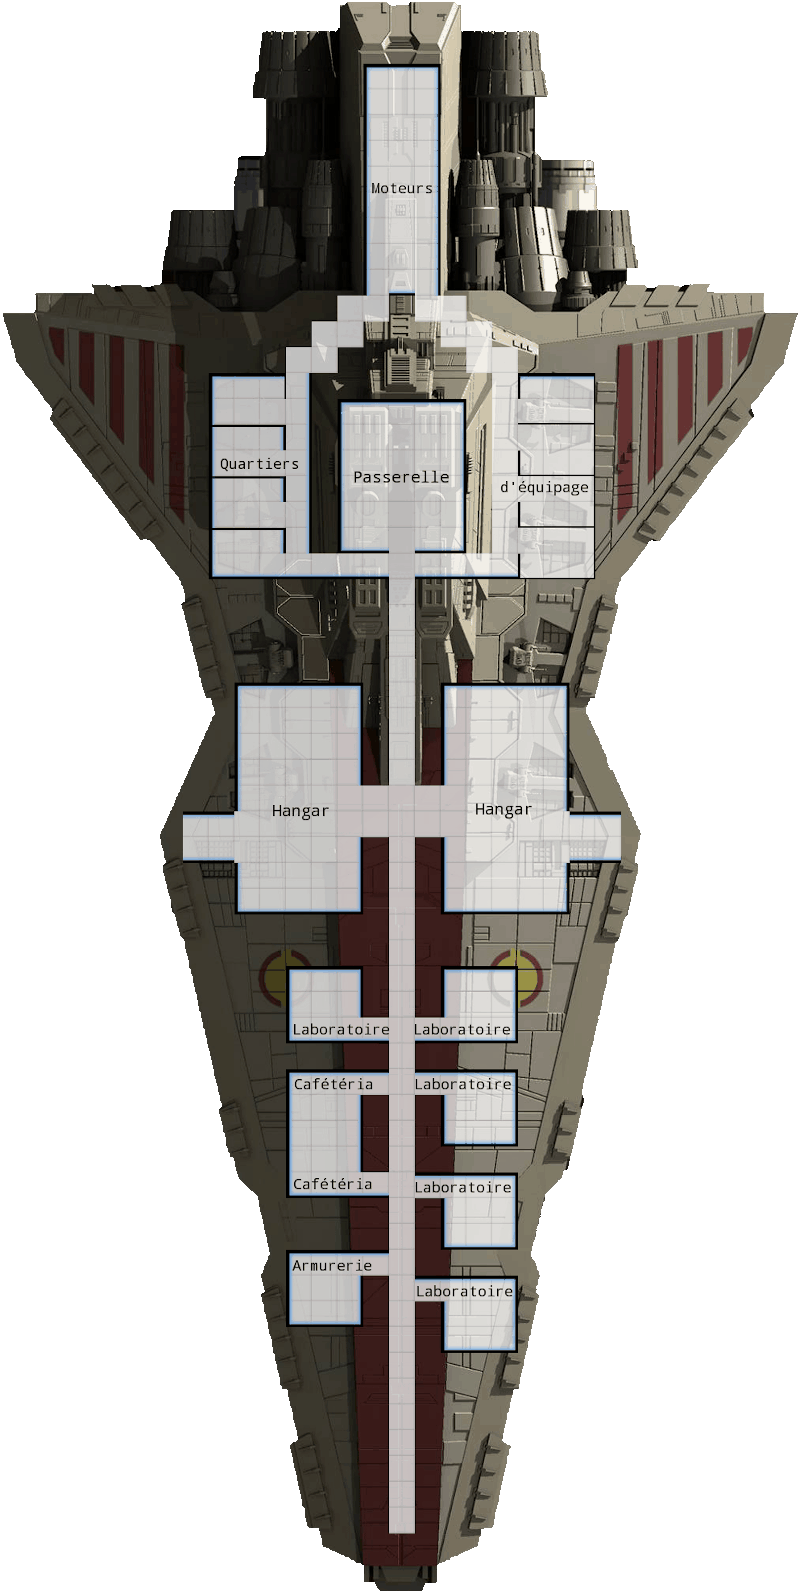
\includegraphics[height=0.87\textheight]{_img/venator-plan.png}
	\caption{Ce n’est qu’une proposition, le plan peut changer à volonté. En annexe, vous trouverez des cases permettant de faire découvrir le vaisseau petit à petit aux héros.}
\end{figure}

\twocolumn

	\section{Les bas fonds de Taris}

C’est parti pour le deuxième volet de la campagne. C’est un épisode qui peut, selon les choix des héros, être assez long. L’épisode précédent était d’environ deux heures, cet épisode peut durer jusqu’à 4 heures selon les directions prises. Il peut aussi être beaucoup plus court si les héros empruntent tous les raccourcis. C’est a vous de doser les ennemis et les choix pour adapter le temps de jeu à ce que vous souhaitez.

\subsection{Prologue}
Nos héros se retrouvent donc dans un Cargo léger YZ-775 sans canons fonctionnels et un message entrant d’une inconnue qui demande à parler à Tinon.
    
Ils ont aussi appris qu’Industrial Automaton sous couvert d’expérimentations de son nouveau modèle, fait des recherches sur un très ancien artefact Sith en provenance de \textbf{Taris}. De plus, s’ils ont réussi à récupérer le droïde, Vyna Anen les attend sur l’avant-poste commercial de \textbf{l’anneau de Kafrene} au Starlord Café. Enfin, ils savent aussi que le vaisseau se dirigeait vers \textbf{Gaulus} pour rejoindre un laboratoire de l’empire où il devait finir des recherches sur l’artefact.

Plusieurs directions s’offrent alors à nos héros.

\subsection{Les bons, les brutes ou les truants}
\begin{quotebox}
    Tinon \emph{(prononcer Taïnon)} c’est toi ? Que se passe t’il ou va tu ?
\end{quotebox}
Le visage d’une jeune femme apparaît sur l’holocomm. Les héros ont le choix de répondre ou non.

Ce point de l’aventure est crucial pour nos héros car ils vont choisir (en connaissance de cause ou non) l’orientation de leurs personnages. En effet plusieurs cas de figures se présentent :

\begin{description}
    \item[\nameref{sec:les-rebelles}] Répondre au message et suivre les consignes des Rebelles (page~\pageref{sec:les-rebelles}).
    \item[\nameref{sec:retour-du-droide}] Ramener le droïde à Vyna Anen (page~\pageref{sec:retour-du-droide}).
    \item[\nameref{sec:refus-d-obtemperer}] Partir pour Taris directement (page~\pageref{sec:refus-d-obtemperer}).
    \item[\nameref{sec:l-empire}] Prendre la direction de Gaulus (page~\pageref{sec:l-empire}).
\end{description}

Tous ses choix amèneront, de toute façon, les héros sur Taris mais le chemin sera différent et par là même leur orientation aussi. Je vais tâcher de décrire les choix possibles sachant que rien n’est écrit dans le marbre et vous pouvez très bien les forcer suivre une route en particulier. C’est un peu le jeu de piste, les choix s’entrecroisent alors faut suivre. Mais une fois de plus rien n’est définitif, les joueurs auront toujours des idées farfelues auxquelles on n’a pas pensé mais je vais essayer de décrire les principales voies possibles, au MJ de diriger les joueurs vers une de ces voies.


\subsubsection{Retour du droïde} \label{sec:retour-du-droide}

Autre choix possible pour les héros, ces derniers, avides de crédits, veulent aller rendre le droïde et récupérer le solde promis pour leur mission. Ils retournent donc sur l’avant-poste commercial dans \textbf{l’anneau de Kafrène} où les attend \nameref{sec:vyna-anen}.

On laisse les héros discuter un peu et réclamer leur due, Vyna acquiesce avec le sourire, leur donne les crédits mais au moment de quitter la pièce, 4 ou 5 \textit{(doser en fonction du niveau de vos joueurs)} Stormtroopers leur barre la route. Attention, à moins que les héros aient anticipé, le premier tour de combat sera pour dégainer.

\begin{quotebox}
    Vous pensiez réellement qu’avec tout ce que vous savez, nous allons vous laisser repartir tranquillement ?\\
    Commencez par me rendre les crédits.
\end{quotebox}

Les héros peuvent tenter de négocier avec Vyna, ce dernier acceptera de les laisser repartir vivant (mais sans crédit) à condition qu’ils retournent sur \nameref{sec:taris} et récupèrent les informations que les scientifiques de Industrial Automaton n’ont pas eu le temps de récupérer. Ils peuvent tenter un jet de Persuasion pour garder les crédits.\\

Si les héros entrent en combat, et qu’ils perdent, on ne les tue pas mais Vyna leur impose de retourner sur Taris et pas de négociation possible. S’ils gagnent, deux cas de figure possibles :
\begin{rebelist}
    \item \textbf{Ils tuent Vyna} Un homme, Chiss, manifestement important en uniforme de l’empire entre dans la pièce en applaudissant. Posément, il félicite les joueurs et leur explique qu’ils ont réussi le test avec brillo. Vyna était devenu gênant pour l’empire et pour l’Odre. Si l’un des héros tente quoi que ce soit il se retrouve désarmé et collé au mur avant d’avoir eu le temps de comprendre. On décroche sur \nameref{sec:l-empire}.

    \item \textbf{Ils laissent Vyna en vie} Une femme (celle qui est apparue sur le holocom du vaisseau) entre dans la pièce avec deux hommes. Les deux hommes emportent Vyna avec eux, en faisant comme s’il était ivre. Et la femme leur fait signe de la suivre vite, elle leur expliquera plus tard. Ils prennent le vaisseau et partent pour la cache des Rebelles. On décroche sur \nameref{sec:les-rebelles} dans la version bien accueillie.
\end{rebelist}

Le \nameref{sec:nimbus} n’est réparé qu’à leur demande, le prix est de 40~000 \crg. Négociable (Persuasion) à 30~000, -10k si relance.


\subsubsection{Les rebelles} \label{sec:les-rebelles}

\begin{quotebox}
    Tinon \emph{(prononcer Taïnon)} c’est toi ? Que se passe t’il où va tu ?
\end{quotebox}

Le visage d’une jeune femme apparaît sur l’holocomm et les héros choisissent de répondre.

\begin{quotebox}
    Mais qui êtes vous et où et Tinon ?
\end{quotebox}
Les joueurs choisissent de raconter leur histoire, ou de mentir, à voir ce qu’ils préfèrent. Lindi leur demande de la rejoindre et leur donne les coordonnées d’une cache de la Rébellion. Si les joueurs ont menti, ils sont accueillis avec suspicion, menacé et tout ce qui va avec, sinon ils sont accueillis normalement avec juste un peu de méfiance. \nameref{sec:lindi-dangon} les invite à la suivre et les interroge jusqu’à ce qu’ils disent la vérité (On part du principe que s’ils persistent à mentir, on bifurque vers l’option \nameref{sec:refus-d-obtemperer}).

Lindi leur explique alors que la résistance a eu vent des recherches menées par l’Industrial Automaton ainsi que des problèmes sur le Pelican. \textbf{Tinon Dystra} avait été envoyé pour tenter de s’infiltrer à bord du Pelican. Mais qu’il n’avait plus donné de nouvelles depuis son arrimage au vaisseau.

Un jet de \textbf{Perception} ou l’utilisation de \textbf{Sens de Force} fera apparaître les sentiments de Lindi envers Tinon et apprendra à nos héros que ces derniers étaient amants.\\

Une fois la discussion terminée, Lindi demande de l’aide aux héros, qu’ils reprennent le travail de Tinon. La première piste à explorer étant \ldots \nameref{sec:taris}.

Le \nameref{sec:nimbus} est réparé gratuitement pendant que les héros discutent.


\subsubsection{Refus d’obtempérer} \label{sec:refus-d-obtemperer}

Les héros veulent se la jouer et décident de partir direct sur Taris. Mais ils ne savent même pas trop ce qu’ils y cherchent. L’hyper-espace est récalcitrant et ne veut pas fonctionner immédiatement. Le temps de regarder, un croiseur sort d’hyper-espace et les arraisonne sans poser de questions. Des soldats de l’alliance (trop pour être combattu) forcent la cloison et entrent dans le cargo, suivis par la femme vue précédemment sur l’holocomm.

\begin{quotebox}
    Où pensiez-vous partir comme ça avec ce cargo ? \\
    \emph{se retournant vers les soldats}, jetez-moi ça en cellule on les interrogera là-bas.
\end{quotebox}

Les héros sont transportés jusqu’à une cache de la Rébellion et jetés en cellule. Au bout de quelque temps, la femme précédemment rencontrée vient les interroger. Ils ont le choix de répondre la vérité ou de mentir. S’ils répondent la vérité, on décroche sur l’option correspondante dans \nameref{sec:les-rebelles}. Sinon ils sont laissés en cellule \ldots

Mais dans la nuit, un mystérieux inconnu s’approche de la cellule sans bruit

\begin{quotebox}
    Je suis envoyé par Vyna Anen, si vous voulez vivre, venez avec moi et pas un bruit.
\end{quotebox}

L’inconnu ouvre leur cellule et les emmène au cargo. Sur le chemin, leur demander des jets de \textbf{Discrétion}. En cas d’échec deux soldats débarquent. Dans le hangar où se trouve le cargo, 4 soldats montent la garde. Soient les héros passent en force et débutent un combat puis vont ouvrir les portes du hangar. Soit ils la jouent furtif, se glissent dans le vaisseau et tirent sur les portes pour sortir du hangar. Ou n’importe quoi d’autres qui leur permet de sortir. Une fois dehors l’inconnu leur transmet des coordonnées. Ils n’ont pas le choix, s’ils font mine de résister, l’inconnu sort une arme et les tiens en joue. Eux n’ont pas d’arme ils sortent de cellule. On décroche ensuite sur \nameref{sec:l-empire}.



\subsubsection{L’empire} \label{sec:l-empire}
Enfin, dernière alternative les héros peuvent vouloir partir pour \textbf{Gaulus} la planète vers laquelle se dirigeait le vaisseau. 

\'A l’approche de la planète, le cargo est arraisonné par un croiseur de l’empire. Les héros sont invités à sortir et une dizaine de Stormtroper les attendent. Ils sont escortés jusque dans un bureau où les attendant \nameref{sec:vyna-anen} et un Chiss en uniforme de gradé de l’empire. C’est ce dernier qui prend la parole.

\begin{quotebox}
    Messieurs (mes dames) nous vous attendions. Asseyez-vous je vous pris. \\
    Alors comment s’est passé cette mission, je vois que tout le monde n’est pas revenu \emph{(sourire aux lèvres)}. 
\end{quotebox}

Le droïde est emmené par deux gardes. Puis le Chiss se présente.

\begin{quotebox}
    Je me présente, je m’appelle \nameref{sec:garan-keggle}, j’ai suivi la mission de loin et je tiens à vous féliciter, vous vous en êtes sorti plutôt bien. Je pensais pas que vous viendriez à bout de l’Amblyope mais j’avoue que le combat était intéressant. Au vu de vos qualités respectives, je souhaiterais que vous partiez pour \nameref{sec:taris} afin de finir la travail \emph{(il jette un regard froid sur Vyna qui en même pas large et baisse les yeux)} nous avons besoin de plus d’information sur la position de l’artéfact.
\end{quotebox}

Si les héros se hasardent à demander un prime, on leur répond que l’empire saura les récompenser sans plus de détail. S’ils sont récalcitrants, on leur explique que c’est pas une proposition que l’on vient de leur faire.


\subsection{Taris} \label{sec:taris}
\noindent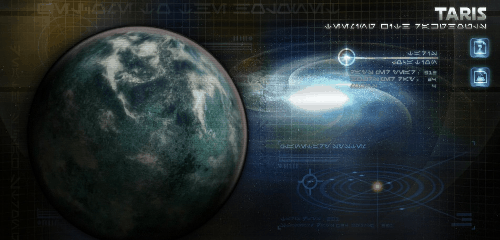
\includegraphics[width=\linewidth]{_img/places/taris.png}
Taris est une planète urbaine, très polluée, de la Bordure Extérieure. Divisée en trois grandes parties en fonction des étages, la Ville Haute, la ville basse et les “bas fonds”, elle abritait autrefois une population gigantesque. Grand pôle économique dans la galaxie, notamment grâce à l’implantation des industries Lhosan, elle joignit la République Galactique peu avant les Guerres Mandaloriennes. Mais après le passage de Dark Malak plus de 4000 ans auparavant la planète a du mal à reprendre vie. Les "bas fonds", qui abritaient toutes sortes de hors-la-loi et de rebus de la société, est la partie de Taris qui s’en est le mieux sortie et c’est pourquoi les ruines marécageuses de Taris sont très dangereuses. La république a depuis implanté un spatioport et une base militaire sur la planète dans l’espoir de la recoloniser mais le processus s’avère lent et compliqué.

Normalement une fois au spatioport, vos héros ne savent pas où aller. Plusieurs choix s’offrent à vous pour les orienter, comme de leur placer un bar bien en évidence sur leur chemin. \'A l’intérieur ils pourront trouver des informations et peut-être même un guide.

Normalement, ils vont se diriger vers le barman. Au pire, c’est le barman qui vient à eux pour leur demander ce qu’ils veulent boire. Ce dernier, un Besalisk, leur explique que l’endroit où ils souhaitent se rendre (les ruines de l’ancien temple Sith) se trouve dans un zone interdite, au c\oe{ur} de la zone de quarantaine \nameref{sec:rakghoul}. Il n’est pas possible de s’y rendre.

Mais un client du bar les accoste et leur dit que moyennant 20~000 \crg il les conduira où ils le souhaitent. Un jet de Persuasion (opposé à la Persuasion de l’inconnu 5) fera descendre la somme à 15~000 \crg.

\begin{paperbox}{Quête annexe (optionnel)}
    Il est possible d’intégrer une petite quête annexe ici histoire de varier les plaisirs. S’ils la réussissent on pourra distribuer +1 XP supplémentaire.

    L’inconnu propose à vos héros de les conduire gratuitement aux ruines s’ils l’aident. Selon l’orientation des joueurs à ce moment, soit:
    \begin{description}
        \item [obscur] Ils aident un contrebandier à Kidnapper une jeune Twi’lek repérée dans un camp de réfigiés pas loin.
        \item [clair] Ils aident un père à délivrer sa fille (adoptive) Twi’lek des mains de contrebandiers.
    \end{description}

    Le roleplay est un peu différent selon la situation mais la quête se déroule de la même façon. Les héros suivent l’inconnu qui s’est présenté entre-temps (\nameref{sec:gil-harend}). Ce dernier les conduit au camp (de réfugiés ou de contrebandier). Un jet de Discrétion réussi par tout le monde permet de s’approcher de la cible. Un jet de discrétion réussi par tous permet de s’extraire de camp sans encombre. Le joueur qui est chargé de transporter la cible à un malus de -2 à son deuxième jet de discrétion.

    Si une Discrétion est ratée par l’un des joueurs, un combat commence. Vos héros se trouve confronté à H -1 contrebandiers/réfugiés (H est le nombre de joueurs que vous avez). Vos héros ont l’initiative sur le premier round. En face, les ennemis ont les caractéristiques \nameref{sec:taris-contrebandier}.

    Attention, \nameref{sec:gil-harend} ne doit pas mourir sinon la quête est un échec et retour au bar. 
\end{paperbox}

\begin{paperbox}{Les aléas du direct}
    Lors du scénar, le droïde était avec les joueurs. Ce dernier connaissait donc les coordonnées des ruines Sith. Il ne leur restait qu’à trouver une guide pour passer les barrages de la zone de quarantaine. L’un des joueurs avec l’Atout \textit{Réseaux} et a souhaité l’utiliser et a fait un jet assez magistral. \nameref{sec:gil-harend} s’est donc trouvé être un ancien camarade du joueur et la quête s’est poursuivie sur cette base.
\end{paperbox}

\subsubsection{Les ruines de l’ancien temple Sith}
\noindent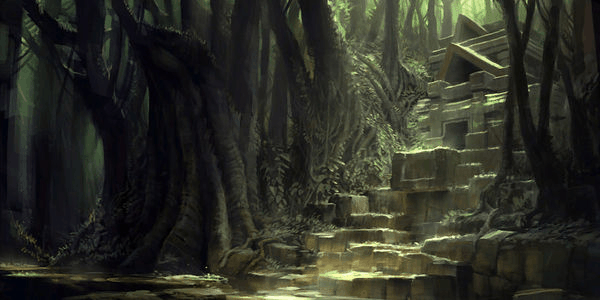
\includegraphics[width=\linewidth]{_img/places/taris-temple-sith.png}

Après plusieurs heures de marche dans les marécages de Taris, le groupe arriver devant les ruines de l’ancien Temple Sith. Le côté obscur de la Force émane du temple dans toutes les directions et l’atmosphère est pesante. D’ailleurs on entend absolument aucun bruit, comme si toute la faune avait déserté la zone. L’entrée est partiellement éboulée mais il reste une ouverture suffisante pour s’y faufiler.

Après être entré dans le temple les héros se retrouvent dans une immense salle, très haute de plafond. Deux rangées de statues de 10m de haut représentent d’anciens seigneurs Sith (Un jet de Connaissance (Sith) permet d’apprendre qu’il s’agit de Tulak Hord, Dakhan Shar, Naga Sadow, \ldots entre autres). Au fond de la salle une fresque murale est gravée sur un monolithe.

Chacun des murs de la pièce (en dehors de celui de l’entrée dans leur dos) possède deux ouvertures vers des pièces.

Devant le monolithe, les vestiges d’un campement de fortune (attention, c’est des vestiges de 3000 ans quand même, heureusement à l’époque on faisait les choses pour que ça dure ;-) ) recouvert de poussière. Une partie de ce campement semble pourtant avoir été remué récemment.

Naturellement, nos héros ne sont pas seuls. 5 \nameref{sec:rakghoul} débarquent et encerclent les héros, s’ensuit une phase de combat.
\\

Une fois les Rakghouls éliminés, les héros peuvent aller observer le monolithe et le campement.

<<insérer le dessin de la fresque>>

Un jet de \emph{Connaissance (Sith)} permet de comprendre la fresque. 

\begin{quotebox}
6000 ans par le passé, un Jedi fut exilé pour ses penchants obscurs et ses expériences interdites sur la vie. Son objectif était, en utilisant le côté obscur, de pouvoir plier la vie elle-même à sa volonté et ainsi acquérir la vie éternelle. En étudiant l’alchimie du côté obscur il parvient à créer un Talisman renfermant son essence et sa volonté. Cet artefact devait, entre autres, lui permettre de prendre possession du corps du porteur du Talisman mais aussi de contrôler les Rakghoul.

Ce Jedi Noir fut tué par un de ses rivaux et durant les décennies suivantes plusieurs Seigneurs Sith se déchirèrent entre eux afin de mettre la main sur ce Talisman. Enfin, l’artefact et son porteur du moment finirent par être tué et enseveli dans ce temple au milieu des bas-fonds de Taris.
\end{quotebox}
Avec une relance, le héros remarquera un étrange renfoncement dans le Monolithe, en forme de triangle.

S’ils ne font pas ce jet ou qu’ils le ratent, ils ne peuvent que tenter d’interpréter la fresque. Après il leur est possible de faire des recherches sur cette fresque dans un temple Jedi ou une bibliothèque. En soi l’histoire n’a pas une grosse importance pour la suite, c’est un bonus pour eux.

Si l’un des héros possède vision de force et s’en sert, il pourra distinguer sur le monolithe un texte, le code des Sith écrit en lettres obscures
\begin{quotebox}
La paix est un mensonge, il n’y a que la passion. \\
Par la passion, j’ai la puissance. \\
Par la puissance, j’ai le pouvoir. \\
Par le pouvoir, j’ai la victoire. \\
Par la victoire, je brise mes chaînes. \\
La Force me libérera.
\end{quotebox}

Il ressentira aussi une impression étrange comme une présence oppressante qui ira même jusqu’à le faire s’évanouir si rate un jet de \textit{Vigueur}.\\

Ensuite avec un jet de recherche sur le campement de fortune, ils trouvent un vieux datapad mais qui a besoin d’être chargé. Dommage, personne n’a de quoi l’alimenter sur lui (sauf si quelqu’un possède l’Atout \emph{Recycleur} et s’en sert). Il faudra trouver le matériel et faire un jet de \emph{Réparer} pour en tirer des informations.

Dans les autres pièces du temple si les héros effectuent une recherche ils ne trouvent rien que des restes de Rakghoul et d’animaux à moitié dévorés.
\'A la sortie du temple, les héros sont attendu de pied ferme par 3 \nameref{sec:taris-contrebandier}. C’est soit les contrebandiers à qui ils ont repris la jeune fille plus tôt qui viennent se rembourser. Soit les amis de \nameref{sec:gil-harend} qui a décidé de les doubler. Dans tous les cas, les contrebandiers veulent récupérer le datapad. Baston\ldots

Une fois débarrassé des contrebandiers, retour au spatioport où ils trouveront de quoi réparer le datapad et en tirer les informations qu’ils cherchent.

\subsection{\'Epilogue}
Le datapad appartenait à un certain \nameref{sec:pulsipher} qui en étudiant les archives du temple Jedi de Taris avait appris l’existence de l’artefact. D’après les informations, Pulsipher a procédé à des excavations et a trouvé le Talisman de Muur. Mais il dut plier bagage rapidement car 3 Jedis appartenant au Cercle de Veille de Taris arrivent pour récupérer le Talisman. Pulsipher quitte alors Taris à bord du Mar’eyce, qui prit la direction de \textbf{Jebble}

\subsection{Progression}
Toujours à titre indicatif~:
\begin{rebelist}
    \item \textbf{1xp} Si ils sont passé par \nameref{sec:les-rebelles} ou \nameref{sec:retour-du-droide}. Dans ces deux cas, les joueurs ont su anticiper les évènements et n’ont pas cherché à tricher.
    \item \textbf{1xp} S’ils ont fait la quête annexe et l’ont réussi, que \nameref{sec:gil-harend} n’est pas mort.
    \item \textbf{1xp} S’ils ont pu traduire le monolithe ou le comprendre correctement.
    \item \textbf{1xp} S’ils se dirigent vers \nameref{sec:jebble} sans que personne ne soit mort.
\end{rebelist}

\subsection{Nimbus} \label{sec:nimbus}
\vspace{-4\baselineskip}
\begin{figure}[h!]
    \centering
    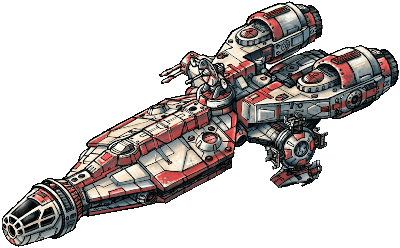
\includegraphics[width=\linewidth]{_img/nimbus.png}
    \caption{Cargo léger YZ-775}
\end{figure}

Le \textbf{Nimbus} est un cargo léger type YZ-775 modifié par l’alliance rebelle. 52~m de long, 8 membres d’équipage, 12 passagers, 400 tonnes da charge utile. Côté armement il dispose de 1 canon turbolaser double, 2 canons-laser doubles, 2 lance-torpilles à proton.

Il appartient initialement à \nameref{sec:tinon-dystra} qui s’en est servi pour infiltrer le \nameref{sec:pelican} lors d’une mission pour l’alliance. Malheureusement, il ne s’en est pas tiré et le Nimbus est resté à quai sur le Pelican. D’où il a servi de nacelle de secours aux héros.

	\section{Laboratoire de Pulsipher}

\subsection{Jebble}\label{sec:jebble}
\noindent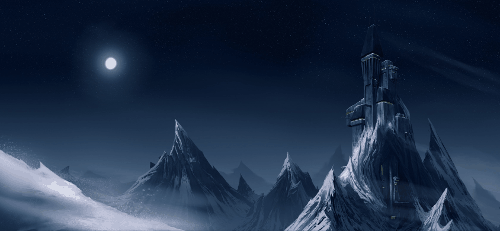
\includegraphics[width=\linewidth]{_img/places/jebble.png}
\'A l’extrémité de la bordure extérieure, complètement gelée à l’image de Hoth, Jebble constituait autrefois le dernier rempart de défense de la République contre les Mandaloriens. Jebble a été le théâtre des évènements concernant le Talisman de Muur, \nameref{sec:celeste-morne} et \nameref{sec:pulsipher}. C’est durant ces évènements que la planète a été bombardé entièrement par la flotte de \textbf{Cassus Fett} afin d’éviter la contagion des Rakghouls. Ce bombardement a fait fondre les glaces de Jebble et les installations de Pulsipher ont coulé dans les eaux bouillonnantes qui ont regelé par-dessus.

Il y a plus de 1~000~ans des mineurs qui cherchaient à exploiter les ressources de la planète, sont tombés sur les installations de Pulsipher, y ont trouvé l’oubliette de Dreya qu’ils ont vendu en tant que «~Boite de Jebble~».

Depuis la planète Jebble a sombré dans le désintérêt le plus complet pour le reste de la galaxie.

\subsection{Astroport de Kriloo City}
Bon, peu importe où ils choisissent de se poser, ils arrivent ici :p.

Kriloo City est une ville de moyenne ampleur. Comme la plupart des villes de Jebble, elle vie essentiellement de l’exploitation des ressources de la planète, elle est surtout composée de mineurs. On y trouve toutes les institutions habituelles, cantinas, bibliothèques, musés, \ldots

\'A leur arrivée, les héros devront trouver des informations sur Pulsipher et ces installations sous la glace. C’est à la bibliothèque qu’ils trouveront cela. Un jet de \emph{Recherche} dans les archives leur apprendra les quelques évènements de l’histoire de Jebble nécessaire à la localisation du laboratoire. Avec une Relance ils lisent quelque chose sur la «~\nameref{sec:boite-de-jebble}~» mais c’est pas bien clair. Ils peuvent aussi demander à la bibliothécaire, une Besalisk avec 4 paires de bras (très pratique pour organiser les documents). Elle leur raconte la même chose que les archives, leur indique où exactement se situe l’entrée de la veine qui mène aux installations enfouies sous la glace. Elle ne leur parle pas de la boite par contre.

Ils ont ensuite le temps de faire des emplettes pour résister au froid (Manteaux, médipac, \ldots) avant de partir pour le laboratoire. Attention, la température de Jebble oscille entre -12° et -30°. Ce qui signifie que tous les héros qui n’ont pas de résistance particulière au froid feront des jets de Vigueur pendant le scénario. Les héros qui n’ont rien acheté pour se couvrir ajouteront un malus de -2 au malus demandé lors du jet. Chaque échec vaudra un niveau de fatigue (cf les règles du froid dans le bouquin de base).

\subsection{En route}
\noindent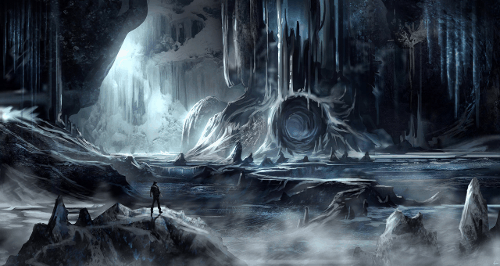
\includegraphics[width=\linewidth]{_img/places/jebble-cave.png}
Nous voilà à l’entrée de la caverne menant aux installations. Avant de s’y engouffrer, tous les héros font un jet de \emph{Vigueur} avec un malus de -2 pour la résistance au froid. En effet, ils ont passé 4 heures à marcher dans la neige par -20° pour arriver jusque-là. Ceux qui ratent prennent un niveau de fatigue.

En entrant dans la grotte, les héros avancent le long d’un étroit tunnel de glace qui s’enfonce dans la glace de l’océan jusqu’à une immense cavité. \'A leur arrivée, des chauves-souries “locale” s’envolent, \ldots bref à vous de décrire. Au fond de la cavité, on distingue des bâtiments pris dans la glace et une entrée creusée à même la glace.

Quand les chauve-souries ont fini de fuir, un grognement se fait entendre dans la grotte et, un \nameref{sec:wampa} surgi de derrière un pilier de glace et s’avance vers eux à grand pas.\\

Une fois le Wampa hors combat, les héros ont le choix de se reposer au près d’un feu pour récupérer de leur fatigue et panser leurs blessures ou d’entrer direct dans le labo.

\subsection{Le laboratoire}

Le laboratoire de Pulsipher possède une IA chargée de sécuriser le laboratoire et d’écarter les intrus. Cette IA, \nameref{sec:lucy-pher} (par ce que ‘\emph{Luc[Puls]ipher}’), est en veille mais les héros vont la réveiller en entrant dans le labo. 

Les héros entrent donc dans le labo de Pulsipher (voir le plan p.~\pageref{sec:plan-labo-pulsipher}). L’entrée est un long sas de plusieurs mètres avant d’arriver dans le laboratoire lui-même. Dans le labo, seuls les sanitaires sont accessibles, tout le reste est verrouillé et doit être soit \textit{Piraté} soit \textit{Forcé}, au choix des héros. Pas de difficulté particulière pour les jets de \textit{Piratage} ou de \textit{Force}, s’ils utilisent un outil approprié pour forcer les portes, ils ont un bonus de +2 au jet de force.

L’ouverture de la première porte déclenche le réveil de Lucy. \'A coté de ce moment il lui faut 5mn (temps IRL) pour sortir de veille et être pleinement activée. Dès que Lucy est activée, le labo se verrouille. Le seul moyen pour les héros de sortir est de débrancher l’ordinateur central.

Lucy dispose de plusieurs moyens pour dissuader les intrus:
\begin{rebelist}
    \item Tous les piratages de portes prennent un malus de -2. Forcer les portes reste possible.
    \item Contrôle environnemental. Lucy peut modifier la température et couper le recyclage de l’air.
    \item Caméras disponibles sur tout le laboratoire (points bleus sur la carte).
    \item Canon Blaster rétractable du plafond (points rouge sur la carte).\\
        \textit{2d10 (1)}
    \item Meute de 5x \nameref{sec:cybercleps}
\end{rebelist}

Donc là les héros sont un peu en galère. La destruction des caméras et Canons dans un secteur rend Lucy aveugle sur le secteur/pièce. Du coup si ça arrive, lâchez les cleps. Sinon laissez les galérer. Les chiens sont là au cas où vos héros s’en sortiraient trop bien. Utilisez-les pour doser la difficulté.\\

Une fois le labo sécurisé, voici la liste des pièces et ce que l’on peut y trouver. Les pièces sont numérotées sur la carte.

\subsubsection{1. Poste Sécurité}
La première pièce à droite en entrant, le PC sécurité, quand il fonctionne donne une vision sur l’ensemble des caméras et des défenses du laboratoire. Il donne un accès au serveur central via un mot de passe. Néanmoins tout y est vieux et obsolète, la moitié des écrans sont brisés les autres clignotent. En mode verrouillage rien n’est accessible depuis ces terminaux.

\subsubsection{2. Salle de pause}
En entrant à gauche, contient des fauteuils des sièges, un distributeur de barres énergétique et de boisson encore rempli. \'A vos héros de voir s’ils se risquent à y goutter. Les barres énergétiques se transforment en poussière à l’ouverture et s’ils gouttent une boisson, ils sont secoués par le goût infâme pendant 10mn.

\subsubsection{3. Débarras}
Un genre de placard de stockage de tout et n’importe quoi. Rien de spécial à y trouver.

\subsubsection{4. Local de contrôle environnemental}
On y gérait toutes les fonctions environnementales de la base. En cas de problème, la base pouvait se verrouiller et devenir autonome. L’air y est recyclé et tempéré depuis les systèmes de ce local. Les serveurs sont indépendants du serveur central mais Lucy peut les commander pour gérer les menaces infectieuses si besoin ou d’autres problèmes de ce genre. Tant que la base n’est pas verrouillée, toutes les commandes sont accessibles. Dès le verrouillage des installations, il faut réussir un \textit{Piratage} pour y parvenir.

\subsubsection{5. Dortoirs}
Les dortoirs des scientifiques du laboratoire. \'A disposition des personnes travaillant dans les installations, ils permettaient de rester dormir ou de se reposer. Les scientifiques n’y habitaient pas à l’année. Rien de spécial à trouver ici non plus.

\subsubsection{6. Garage}
Le garage est une vaste pièce. Il reste un genre de Jeep Rover en bon état mais la batterie est morte et les portes du garage sont condamnés par la glace. On trouve dans le garage divers outils et des pièces de rechange pour véhicules, ainsi que 2 Medipacs.

\subsubsection{7. Laboratoire Principal}
Pièce centrale des installations, c’est ici qu’étaient faites toutes les recherches. Elle est équipée de tout le matériel d’analyse dont un scientifique pouvait rêver \ldots il y a 3~000 ans. Malgré l’age du matériel il reste fonctionnel et la sortie de veille des installations a rétablie l’alimentation. Un \textit{Soin} effectué dans cette pièce avec les appareils présents est accompagné d’un bonus +2 et ne consomme pas de Medipac.

\subsubsection{8. Zone de quarantaine}

\begin{wrapfigure}{r}{0.4\linewidth}
    \vspace{-5\baselineskip}
    \centering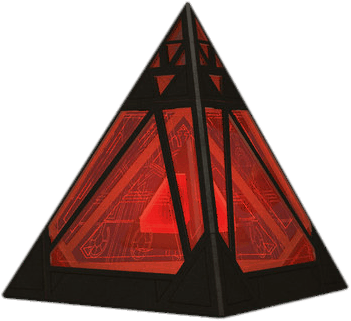
\includegraphics[width=\linewidth]{_img/holocron-sith.png}
    \vspace{-2\baselineskip} 
\end{wrapfigure}
Lieu où étaient stockés les matières dangereuses ou soupçonnées dangereuses. On y trouve un tas de containers étanches, certains ouverts d’autres scellés. Des étagères et des réfrigérateurs qui fonctionnent mais la chaîne du froid n’a certainement pas été respectée.

On trouvera dans cette pièce un Holocron Sith, créé par \nameref{fig:karness-muur} lui-même. Cet holocron est pour l’instant inutilisable. Il faut une affinité avec la Force pour l’ouvrir et un genre de clé mentale. Karness a verrouillé son Holocron pour qu’il ne tombe pas dans les mains de ces ennemis. \'A moins de réussir un jet de \textif{Connaissance (Sith/Jedi)} les joueurs ne voient qu’un objet triangulaire. Ceux qui ont \textit{Vision de Force} ressentent l’émanation obscure de l’objet.

\subsubsection{9. Centre de contrôle}
Un ensemble de terminaux sont disponibles dans cette pièce. Tant que Lucy est active, ils sont tous verrouillé et non Piratable.

\'A partir du moment où Lucy est désactivée, les terminaux donnent accès à toutes les informations du Labo, sans \textit{Piratage}. Deux informations sont importantes~:
\begin{rebelist}
    \item L’\nameref{sec:oubliette-de-dreypa} est la clé pour se débarrasser du Talisman de Muur
    \item L’\nameref{sec:talisman-jebble}
\end{rebelist}

\subsubsection{10. Central Informatique}
Le centre nerveux de Lucy. C’est dans cette pièce que se trouve le seul et unique terminal d’accès au programme de Lucy. Si/Quand les héros parviennent à cette pièce, les \nameref{sec:cybercleps} sont systématiquement lâchés. Un \textit{Piratage} est possible. Un succès désactive Lucy, une \textit{Relance} reboute Lucy et permet de la contrôler pour effectuer plus vite les recherches dont les héros ont besoin.

\'A partir du moment où les héros entrent dans la pièce, une phase de combat commence. Les héros peuvent choisir de repousser les chiens le temps que l’un d’eux parvienne à \textit{Pirater} Lucy. Si c’est le cas, le joueur en question reçoit une carte comme les autres mais à son tour il fait un jet de \textit{Piratage}. Dès que le \textit{Piratage} est réussit les chiens sont hors combat.

\subsubsection{Canons \& Caméras}
Sur le \nameref{sec:plan-labo-pulsipher} sont disposé les Caméras (triangles verts) et les tours de canons (carrés rouges). Les caméras sont rotatives. Tous ce qui n’est pas dans le champ d’une caméra n’est pas visible par Lucy.

Les canons aussi sont rotatifs, ils possèdent les caractéristiques de \textit{Canon blaster embarqué}~:
\begin{itemtable}[ X c c c c ]
    \textbf{Type} & \textbf{Porté} & \textbf{Dégâts} & \textbf{Résistance} \\
    Canon blaster & 600            & 2d10  (1)       & 10 \\
\end{itemtable}

\onecolumn
\subsection{Plan du labo de Pulsipher}\label{sec:plan-labo-pulsipher}
\begin{figure}[!h]
	\centering	
	\begin{tikzpicture}[overlay, anchor=north]
		\node at (0,0) {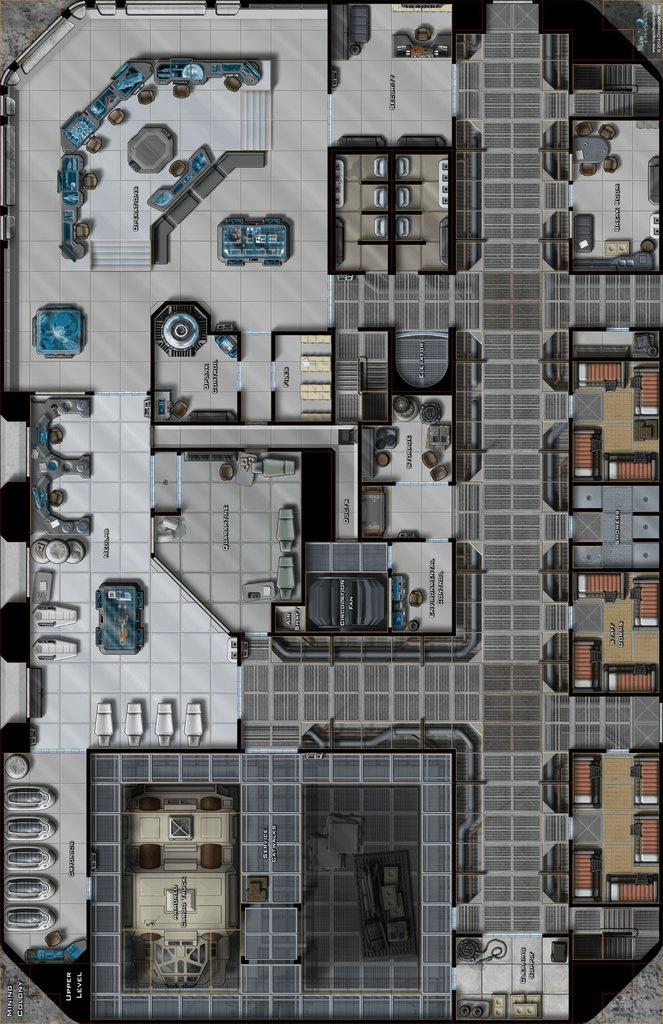
\includegraphics[height=0.94\textheight]{_img/places/labo-pulsipher-map.png}};
		\node at (0,-0.4) {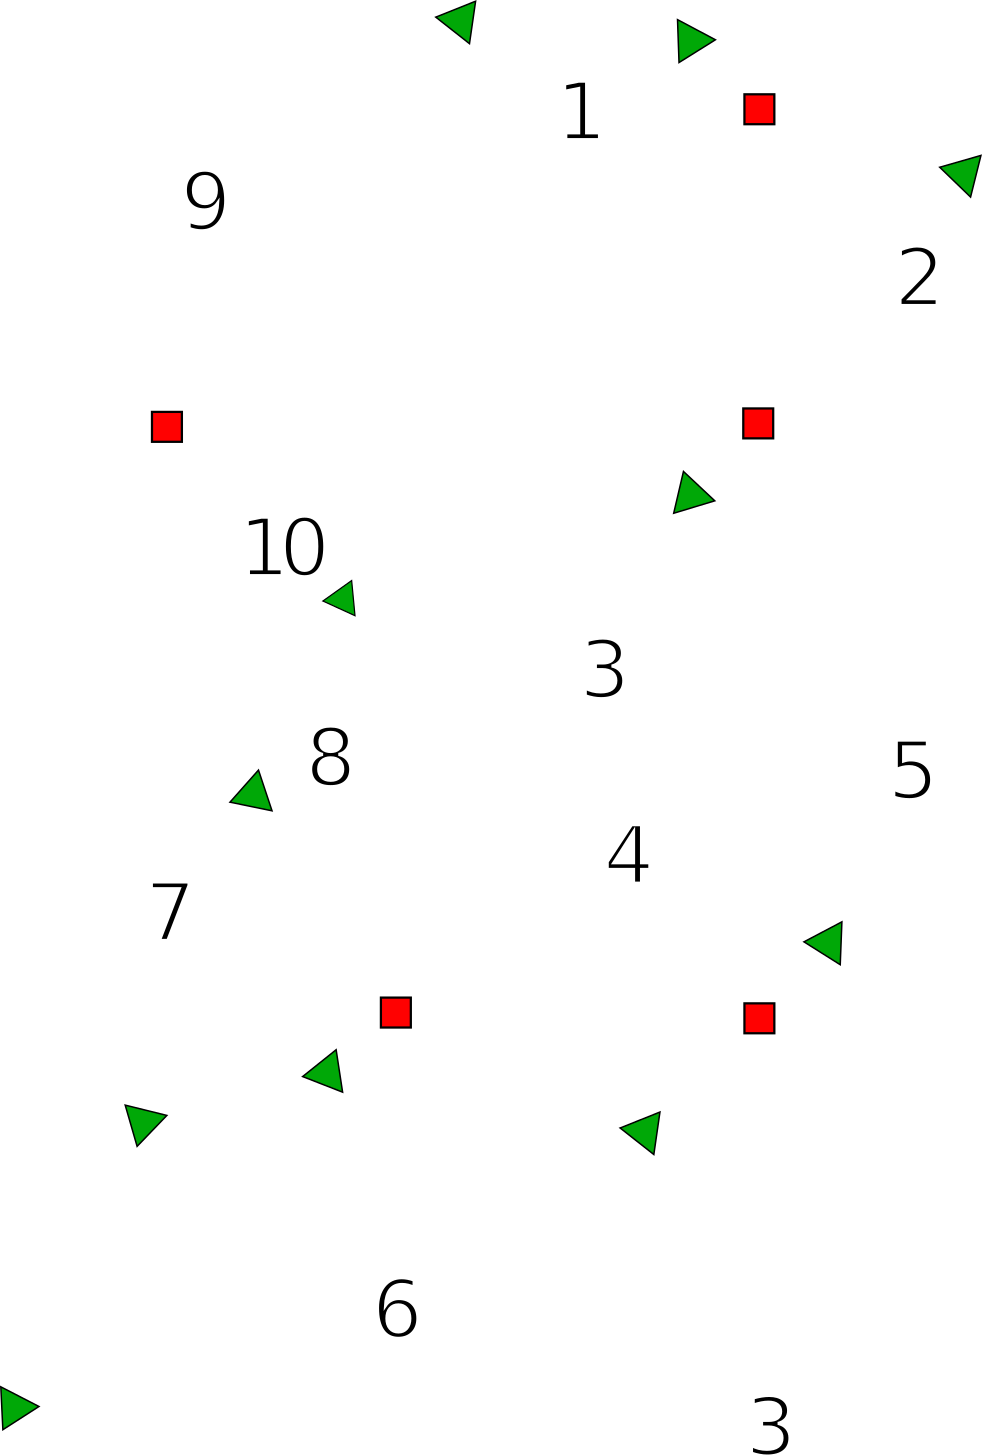
\includegraphics[height=0.89\textheight]{_img/places/labo-pulsipher-layers.png}};
	\end{tikzpicture}
\end{figure}

\twocolumn

\subsection{Oubliette de Dreypa}\label{sec:oubliette-de-dreypa}
Au début de l'Empire Sith, un Seigneur Sith du nom de Lord Dreypa créa, probablement grâce à la sorcellerie sith, une oubliette. Celle-ci avait la capacité de plonger son occupant dans une forme de stase tout en le maintenant conscient et en le soumettant à des tortures. Dreypa la destinait à son rival, le Seigneur Sith Karness Muur, mais ne put jamais mener son projet à terme, du moins de son vivant… 

\subsection{Histoire du Talisman sur Jebble}\label{sec:talisman-jebble}
Les données trouvées dans les ordinateurs du labo apprennent aux héros que \nameref{sec:pulsipher} a voulu s’emparer du pouvoir du Talisman pour créer son propre clan Mandalorien. Mais le Talisman a sa propre conscience, celle de \nameref{fig:karness-muur}. Et son but à lui est de trouver un hôte dont la sensibilité à la Force est le plus élevé possible. Il quitta donc Pulsipher pour s’emparer de \nameref{sec:celeste-morne}, une Jedi venu arrêter les agissements de Pulsipher.

Céleste parvint à se maîtriser juste assez longtemps pour permettre à \textbf{Zayne}, son Padawan, de l’enfermer dans l’\nameref{sec:oubliette-de-dreypa} le temps que ce dernier trouve une solution pour la débarrasser du Talisman. Malheureusement pour eux, c’est à ce moment que \textbf{Cassus Feth} un chef Mandalorien de l’époque, bombarda toute la zone du Labo afin d’endiguer la maladie des rakghouls. Les glaces autour du labo fondirent et engloutirent le Labo et l’oubliette avant de regeler par-dessus.

La population locale connaissait l’oubliette sous le nom \testbf{Boite de Jebble}\ldots 

C’est là que s’arrête les données de l’ordinateur.

\subsection{La Boite de Jebble}\label{sec:boite-de-jebble}
Si nos héros retournent à Kriloo City, et qu’ils posent des questions sur la \textbf{Boite de Jebble}, n’importe qui leur parlera de la légende. Légende qui date d’au moins 1~500~ans. Une boite trouvée 1~km sous la glace, impossible à ouvrir, impossible à scanner, qui a été étudié plusieurs années sans le moindre résultat et qui a fini par être vendu à on ne sait plus qui. On dit que seul un Jedi pourrait l’ouvrir mais il y a un prix à payer. C’est la boite de Pandore version Jebble !

\subsection{\’Epilogue}
Nos héros n’en apprendront pas plus sur Jebble. Ils doivent maintenant se mettre à la recherche de la \textbf{Boite de Jebble}. Pour faciliter la transition avec le prochain scénar, à leur retour au Nimbus, les héros reçoivent un message de leur faction (Alliance ou Empire) leur demandant où ils en sont de leur recherche.

\subsection{Progression}
Toujours à titre indicatif, ce scenario était un peu moins velu que le précédent, c’est seulement 2xp que je distribue aux joueurs.


	\section{C’est dans la boite}


\subsection{Au rapport !}
Nos héros quittant Jebble son contacté par leur faction.

\subsubsection{Empire}
\begin{quotebox}
    \nameref{sec:garan-keggle}: Au rapport~! Comment avancent vos recherches sur l’artefact~?
\end{quotebox}
Les joueurs racontent\ldots
\begin{quotebox}
    \nameref{sec:garan-keggle}: La "Boite de Jebble"\ldots Ça ne me dit rien~! Mais allez voir \nameref{sec:fane-peturri} sur \textbf{Muunilinst}, c’est un historien de l’Empire, ami de notre Empereur, il pourra certainement vous aider. Je vais le prévenir de votre visite et je vous transfère ses coordonnées.
\end{quotebox}

Les héros se rendent donc sur \textbf{Muunilinst} (normalement) et rencontrent \nameref{sec:fane-peturri}. Ce dernier les invite chez lui, leur offre le thé et les reçoit bien.
\begin{quotebox}
    \nameref{sec:fane-peturri}: Garan m’a prévenu de votre arrivée, mais il ne m’a pas dit quel était le but de votre visite~? En quoi puis-je aider l’empire~?
\end{quotebox}
Les héros devraient donc lui parler de la fameuse boite de Jebble qui est en réalité \nameref{sec:oubliette-de-dreypa}.

\begin{quotebox}
    \nameref{sec:fane-peturri}: Il me semblait bien qu’il y avait un rapport entre l’oubliette et cette Boite~! Il y a quelque temps, suite à une réquisition d’\oe{uvres} d’art pour le compte de l’Empire, je suis tombé sur un enregistrement holo qui parlait de cette boite. D’après ce que disait l’enregistrement, mais il date maintenant de plusieurs mois, la \textbf{Boite de Jebble} se trouve sur le \nameref{sec:uhumele} un cargo qui verse dans le commerce et la contrebande de babioles diverses. Son capitaine, \nameref{sec:schurk-heren} est un Yarkora qui se méfie de tout le monde en général et en particulier de l’Empire. Dites-lui que vous êtes des amis de "\textbf{\nameref{sec:uhumele-janks}}" mais il n’est pas idiot donc prenez ce dossier sur Janks et étudiez le avant de vous faire passer pour ses amis.

    Le dernier port d’attache que je lui connais est \textbf{Pizkoss}, il est certainement en train de dépenser ses crédits chez \nameref{sec:queen-jool}.
\end{quotebox}

\subsubsection{Rebelion}
\begin{quotebox}
    \nameref{sec:lindi-dangon}: Bonjour, je viens aux nouvelles, comment se passe la recherche de l’artéfact~? Vous avez besoin de quelque chose~?
\end{quotebox}

Les joueurs racontent\ldots

\begin{quotebox}
    \nameref{sec:lindi-dangon}: La \textbf{Boite de Jebble}, ça me dit quelque chose, attendez une seconde\ldots 

    \textit{Lindi disparaît de l’écran un instant puis revient}

    \nameref{sec:lindi-dangon}: Effectivement, un Jedi en parle dans un de ses rapports. \nameref{sec:dass-jennir}, il n’est pas très précis dans son rapport, mais vous devriez aller le voir. Il est en retraite sur \textbf{Muunilinst}. Je vous fais suivre les coordonnées où vous le trouverez, soyez respectueux et diplomates~! Rappelez-vous que c’est un Jedi~!
\end{quotebox}

Les héros se rendent donc sur \textbf{Muunilinst} (normalement) pour rencontrer \nameref{sec:dass-jennir}. Dass Jennir se montre tout d’abord froid et distant
\begin{quotebox}
    \nameref{sec:dass-jennir}: C’est pour quoi~? Si c’est encore pour réparer votre moissonneuse, revenez plus tard, je suis occupé là.
\end{quotebox}

Aux héros de se montrer diplomate pour l’amadouer~! Quand c’est fait. Ils lui parlent de la Boite de Jebble. En entendant ce nom, le visage de Dass Jennir marque un sentiment de souffrance et de regret. C’est manifestement un souvenir douloureux pour lui.
\begin{quotebox}
    \nameref{sec:dass-jennir}: Oui, je me souviens de ça~! Je ne l’ai pas vu personnellement, mais elle faisait partie de l’inventaire de l’\nameref{sec:uhumele} quand je suis passé à son bord pour une mission. L’équipage du vaisseau avait à son bord cette chose, aux dernières nouvelles ils partaient sur \textbf{Pizkoss} pour tenter de trouver un acheteur pour cette cargaison.

    Vous devez savoir que déjà à l’époque, l’Empire recherchait ardemment cette cargaison, c’est d’ailleurs ce qui explique qu’il ne l’ai toujours pas revendue. 

    Le capitaine du cargo s’appelle \nameref{sec:schurk-heren} je vais vous dire où le trouver sur \textbf{Pizkoss} mais je ne viendrais pas avec vous, j’en ai fini avec tout ça.
\end{quotebox}

Quand \nameref{sec:schurk-heren} fait escale sur \textbf{Pizkoss}, il a l’habitude de dépenser ses crédits chez \nameref{sec:queen-jool}.

\newpage
\subsection{Pizkoss’ Paradise}
Pizkoss était un Monde du Noyau. En tant que tel, le commerce y est très prospère et on y retrouve à peu près toutes les races possibles. Toutes sortes de transaction et ont lieu des plus légales aux plus douteuses. En tant que planète du noyau elle est surveillée par l’Empire.

\nameref{sec:queen-jool} est la propriétaire d’une cantina libertine sur \textbf{Pizkoss}, le \textbf{Paradise}. C’est un club "select" où l’on ne rentre que sur invitation. Il ne faut pas chercher à rentrer de force au risque de se faire expulser violemment et d’attirer par la même l’attention de l’Empire. Diplomatie et astuce (déguisement, soudoiement, propositions indécentes \ldots) sont de rigueur. Une fois à l’intérieur, attention de ne pas faire de vagues~! Au moindre problème, vigiles et \nameref{sec:storm-trooper}s débarquent et enferment tout le monde.\\

\noindent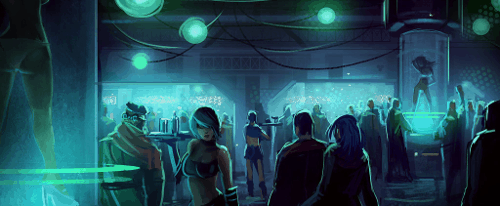
\includegraphics[width=\linewidth]{_img/places/paradise-club.png}\\

\'A l’intérieur la salle se présente comme un stripbar classique. Un bar sur la droite, une estrade au fond avec un podium qui avance sur la moitié de la pièce. Des îlots plus privés tout au tour et des salons privatif sur la gauche. 

Les héros ne savent pas à quoi ressemble \nameref{sec:schurk-heren} ils n’ont que son nom, à eux de le retrouver. En vrai il se trouve dans l’un des salons privés où il profite d’une danse avec \textbf{Na’tuna}, une charmante Twi’lek en tenue légère.

Quand les héros rentrent dans le salon, Schurk est un peu surpris, Na’Tuna reste imperturbable, professionnalisme avant tout.

\begin{quotebox}
    \nameref{sec:schurk-heren}: Ben faut pas vous gêner~! Décidément tout se perd, les bonnes manières y compris~! Je ne sais pas ce que vous me voulez mais vous ne pensez pas que ça peut attendre que la dame est terminée~?
\end{quotebox}

Gérez Schurk en fonction du comportement de vos héros, quand ils se mettent à discuter~:

\begin{quotebox}
    \nameref{sec:schurk-heren}: Bon, maintenant que l’on est entre nous, en quoi puis-je vous aider ?\\
    \textit{\textbf{Joueurs}}: \ldots\\
    \nameref{sec:schurk-heren}: Humm, alors comme ça cet inestimable et antique coffre vous intéresse ? C’est fâcheux, figurez-vous que je viens tout juste de le promettre à un client fortuné. Il serait vraiment très déçu si je lui faisais faux bon.\\
    \textit{\textbf{Joueurs}}: \ldots\\
    \nameref{sec:schurk-heren}: Cependant vous m’êtes sympathique~! Il se pourrait que je vous dise où se trouve la cargaison. Si vous êtes assez rapide, vous pourrez la récupérer avant mon autre client. Je n’ai pas encore rencontré mon client pour la transaction, ça vous laisse le temps de me rendre un petit service.\\
    \textit{\textbf{Joueurs}}: \ldots \\
    \nameref{sec:schurk-heren}: Mais vous êtes des amis de \textit{[\textbf{Dass Jennir}|\textbf{Janks}]}, je ne me vois pas vous refuser ça~! Il se trouve que je n’ai pas une confiance aveugle en ce client. Il est connu pour être un criminel et je m’attends à ce qu’il essaye de me doubler. Dans ces conditions, je vous propose d’assister à la transaction de loin. Si ça tourne mal, on se débarrasse de lui et je vous fais la cargaison à prix d’ami.

    Si tout se passe bien, vous connaîtrez l’emplacement de la cargaison et n’aurez qu’a vous y rendre avant eux. C’est ce que je peux vous proposer de mieux.
\end{quotebox}

Peu importe de la prix que vous négocierez avec les héros il n’y aura jamais besoin de le payer.
\begin{paperbox}{Songes d’Uhumele}
    \'A noter que si vos héros ont fait le scénar \citetitle{swr-songes-uhumele}, ils connaissent les membres de l’Uhumele ainsi que leur aventure avec \nameref{sec:dass-jennir} et ils ont le droit d’en jouer. Ils y sont même encouragé.
\end{paperbox}
\subsection{La transaction}

La transaction à lieu dans un entrepôt à l’extérieur de la ville. L’Uhumele est stationné à l’extérieur, nos héros restent dans le cargo alors que le capitaine et son équipage partent avec un fausse cargaison pour traiter avec le client. Les héros distinguent ce qu’il se passe de loin.

Tout semble bien se passer mais brusquement le client, un \textbf{Ishi Tib} apparemment, sort une arme. Schurk-Heren tente d’en faire autant, mais elle lui est oté des mains par un tir de blaster venant de sa droite en hauteur. Depuis le vaisseau, les héros voient sortir une douzaine d’hommes armé de \textit{Fusil Blaster} qui encercle l’équipage.

Les héros peuvent ici choisir d’entrer dans le combat ou non. Le nombre d’adversaire à combattre est important et doit les obliger à mettre au point une stratégie de repli permettant de sauver au moins l’un des membres d’équipage, vu qu’ils ne savent toujours pas où se trouve la cargaison. Si les héros entrent dans le combat, laissez passer quelques tours de combat, quand les héros commencent à souffrir un peu, ou s’ils s’enfuient, passez à la suite.\\

Donc au bout d’un moment, un vaisseau apparaît au-dessus de l’entrepôt et fait exploser le toit (Si tous les joueurs sont dans l’entrepôt, ils ne le voient pas arriver). Le vaisseau prend tout le monde pour cible, peu importe le camp, pendant qu’un rayon tracteur fait main basse sur la fausse cargaison.
Les hommes du \textbf{Ishi Tib} sont encore nombreux mais sont distrait par le vaisseau qui vole leur cargaison.

Le capitaine de l’Uhumele prend un tir dans l’épaule qui le blesse gravement. Deux autres de ses équipiers se font blesser à leur tour. Voyant la situation mal tourner, les deux blessés demandent aux héros et au reste de l’équipage de prendre leur capitaine et de partir se mettre à l’abri pendant qu’ils couvrent leur fuite. Les héros parviennent à atteindre le vaisseau mais les hommes de l’\textbf{Ishi Tib} se ressaisissent et les héros voient les deux hommes d’équipage capturés par le \textbf{Ishi Tib}.

Une fois à bord, \textbf{Schurk-Heren} commande au vaisseau de dégager et de mettre le cap sur \textbf{Pizkoss}. Une fois en sécurité, 
\begin{quotebox}
    \nameref{sec:schurk-heren}: Ce vaisseau, je le connais, c’est celui du bras droit du \textbf{Ishi Tib}. Il aura eu les yeux plus gros que le ventre et aura voulu la cargaison pour lui seul.\\
    \nameref{sec:schurk-heren}: Je dois partir secourir mes hommes. S’ils sont interrogés, ils finiront par avouer que la cargaison était un leurre et il ne faudra pas longtemps avant qu’ils soient forcés de donner l’emplacement de la vraie. Il faut la récupérer au plus vite. Vous irez chercher la cargaison pendant que nous irons secourir le reste de mon équipage.\\
    \nameref{sec:schurk-heren}: La cargaison se trouve dans un champ d’astéroïdes, je vous transfère les coordonnées.
\end{quotebox}

Les joueurs reprennent leur vaisseau sur \textbf{Pizkoss} et partent vers les coordonnées données par \textbf{Schurk-Heren}.

\subsection{Le champ d’astéroïde}
\noindent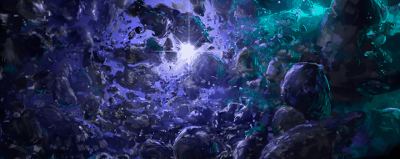
\includegraphics[width=\linewidth]{_img/places/asteroid-field.png}\\

Donc nos héros s’en vont chercher ce pour quoi ils sont venus, \nameref{sec:oubliette-de-dreypa} alias "la boite de Jebble". Mise à l’abri dans un champ d’astéroïdes par \nameref{sec:schurk-heren}.

Le champ d’astéroïde oblige les vaisseaux à sortir d’hyper-espace au large des coordonnées indiquées par Schurk. Dès la sortie, tous les voyant du \nameref{sec:nimbus} passent au rouge. En effet, ils ne sont pas seuls sur les lieux, une \nameref{sec:empire-corvette} est présente sur la zone. Quelques instants après leur arrivée, 4 \nameref{sec:tie-fighter} sont largué de la corvette et se dirige vers le Nimbus pendant que la corvette s’engouffre dans le champ d’astéroïdes.

Un affrontement spacial s’engage entre le \nameref{sec:nimbus} et les 4 \nameref{sec:tie-fighter}. \textit{Les spécificités offencive et défencives des différents vaisseaux sont disponibles dans le \nameref{sec:bestiaire} et dans la section \nameref{sec:nimbus}}.\\

Une fois les 4 chasseurs explosés, les héros se précipitent (en principe) sur la zone où se trouve l’oubliette. Un cargo léger est en train de récupérer la cargaison de l’Uhumele quand le Nimbus arrive à portée de la corvette.

Les héros peuvent engager le combat, mais entre les dégâts encaissés contre les chasseurs et le fait que la corvette est mieux armée, le combat n’est pas égal. Ils peuvent prendre le cargo pour cible mais s’ils parviennent à l’exploser, la corvette utilisera un rayon tracteur pour récupérer la boite.

Au final, la corvette prendra la fuite sans demander son reste et les héros n’ont que leurs yeux pour pleurer.

\subsection{\'Epilogue}
C’est pour une fois, un scénar qui ne se termine pas bien. On peut pas toujours gagner !

Pour l’XP, entre \textbf{2 et 3 XP} selon le jeu et la cohérence des joueurs.

\clearpage
\subsection{l’Uhumele}\label{sec:uhumele}
\noindent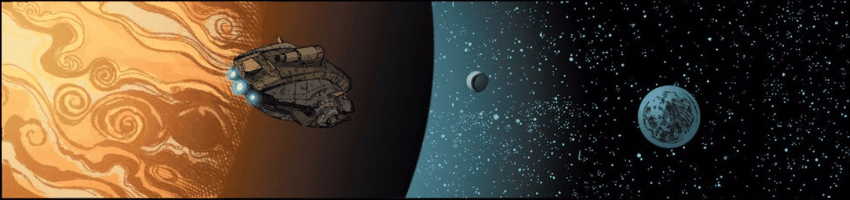
\includegraphics[width=\textwidth]{_img/uhumele-pano.png}

L'Uhumele est un vaisseau cargo de classe inconnue, actif notamment pendant et après la Guerre des Clones. Son capitaine est le Yarkora Schurk-Heren. On ignore quand et dans quelles conditions Schurk-Heren devint capitaine de l’Uhumele et comment son équipage le rejoignit. Ce qui est sûr, c’est qu’il a de bonnes raisons de détester la République et de craindre l’Empire qui lui succède.

L’Uhumele est avant tout un vaisseau de contrebande, comme un bon nombre de cargos en apparence en règle. De ce fait, il est doté d’un armement susceptible de pouvoir le sortir des situations délicates dans lesquelles il se fourre. L’une de ces armes est un bras rétractable situé sous le ventre de l’appareil, au bout duquel se trouve une petite tourelle blaster, ressemblant à celle des Canonnières clones. Bien que cette tourelle permette d’avoir un très vaste angle de tir, elle rend la situation du tireur précaire car très exposé. 

\subsubsection{Janks}\label{sec:uhumele-janks}
\hspace{12em}
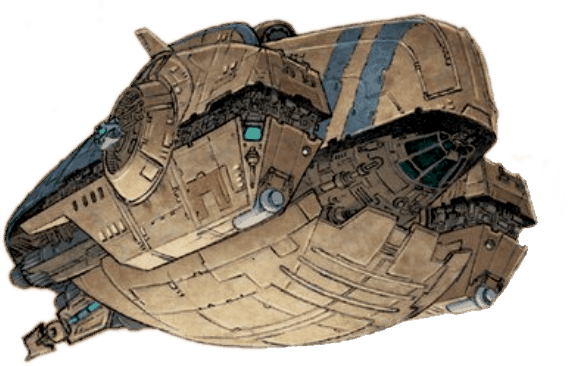
\includegraphics[width=0.8\textwidth]{_img/uhumele.png}
%   Ici une idée est qu'au moment de quitté la planète pour l'étape suivante, les héros se retrouvent pris au piège par des troupes de l'empire qui on pris leur vaisseau en otage. Histoire de varier l'aventure. On peut même se mettre une petite baston spaciale.

% La suite c’est qu'il faut retrouver la boite avant que quelqu'un d'autre ne mette la main dessus (l'Empire ou un rival de Palpatine). Mais c'est raté, c'est les méchant d'en face qui récupèrent en premier et qui l'ouvre.

% scénario suivant et final, les méchant tendent un piège aux héros grace à Céleste mais les gentils parviennent à libérer Celeste et à remettre l'amulette dans l'oubliette. Cette dernière est récupérer par la faction des héros et conservée à l'abris.
	\section{Dos au Muur}
On attaque ici le cinquième et dernier chapitre de la saga.

\subsection{Résumé des épisodes précédents}
Le camp opposé (l’empire pour les gentils et l’alliance si vos héros sont avec Dark Vador) a récupéré l’\nameref{sec:oubliette-de-dreypa} au nez et à la barbe de vos héros qui sont donc bien dégoutté. S’ils ont bien joué, vos héros ont trouvé l'Holocron de Muur dans le laboratoire de \nameref{sec:pulsipher}. Enfin, vos héros savent ce que contient l’oubliette.

Ils vont donc errer un moment dans l’Univers à la recherche d’informations qui pourraient les mener à l’oubliette perdue. Selon que vos joueurs se montrent imaginatif ou pas sur la recherche, abrégez ou non la séquence par un appel de leur hiérarchie qui aura à leur faire part d’une. Si vos joueurs se montrent imaginatif faites leur trouver la dite information par eux-mêmes.

\subsection{Sur la piste}
\paragraph{Empire}
Si vos héros sont à la solde de l’Empire, l’information qui finie par leur parvenir est que des espions infiltrés ont découvert au péril de leur vie que les rebelles ont amené sur une base reculée de l’alliance, une cargaison très spéciale et que depuis seul le personnel fortement accrédité est autorisé à circuler dans la zone de stockage de la cargaison.

La base rebelle se trouve sur la lune IV de Yavin. Les rebelles sont établis dans ce système depuis plusieurs mois. La quatrième lune de Yavin est une lune forestière avec une végétation dense offrant un bon camouflage aux bâtiments installés sous la canopée. La lune possède plusieurs installations distante les unes des autres de plusieurs centaines de kilomètres. La fameuse cargaison est entreposée et sans doute étudiée dans l’installation la plus au Nord et la plus éloignée de toutes les autres.

\paragraph{Alliance}
Si vos héros se sont enrôlés dans la résistance, c’est un peu la même histoire. L’information qui leur parvient est que l’Empire à fait porter sur une lune de Lothal une cargaison et que depuis le bâtiment où est entreposée la cargaison est verrouillé. 

Sur l’une des lunes de Lothal, l’Empire possède une base militaire. La lune est de type désertique. Pas de végétation ni d’eau, seulement une atmosphère un peu raréfiée. La cargaison est entreposée 100~km au Nord de la base dans une zone qui depuis est fermée à tous les soldats non autorisés.

\paragraph{Commun}
Dans tous les cas, les héros sont prévenus que le camp adverse s’emploie à ouvrir l’Oubliette mais que pour l’instant il n’y est pas parvenu.

\'A ce moment de l’histoire, vos héros devraient sentir (ou non) le piège, il leur faut donc un plan. Ils savent que dans l’oubliette se trouve \nameref{sec:celeste-morne}, une puissante Jedi et, qui plus est, possédée par le Talisman de Muur, un non moins puissant Sith ! Le combat, si combat il doit y avoir, s’annonce un peu difficile. \'A vous de leur faire comprendre, s’ils ne le ressentent pas spontanément, qu’y allez sans un plan pour libérer Céleste du Talisman n’est rien de plus qu’un suicide collectif.

\subsection{Man with a plan}
C’est là qu’intervient l’Holocron de Muur.

S’ils ne l’ont pas trouvé, hé bien c’est qu’ils ont mal joué ! La meilleure solution est encore de leur faire comprendre qu’il leur manque une pièce du puzzle et qu’ils doivent retourner sur \nameref{sec:jebble} chercher l’Holocron. Par exemple en leur rappelant que le datapad de \nameref{sec:pulsipher} faisait référence à un objet triangulaire.

S’ils ont l’Holocron avec eux, il est temps de leur faire comprendre que c’est un élément important de l’histoire et qu’il va falloir trouver comment l’ouvrir. Pour l’ouvrir ils vont devoir retourner sur \nameref{sec:taris} dans les ruines de l’ancien temple Sith. Sur le Monolithe en y regardant d’un peu plus prêt on trouvera un emplacement triangulaire où l’Holocron entre à la perfection. Cette fois, on leur facilite le passage, pas de gros boss ni de complication particulière. C’est comme dans les jeux une fois que la zone est visitée elle est sécure. Et puis l’objectif de la mission n’est pas de refaire le scénario 2.

\newpage
\begin{paperbox}{Comment les amener sur Taris ?}
Quelques idées sur comment les amener à retourner sur Taris pour ouvrir l’Holocron. Car ce dernier étant verrouillé sur l’esprit de Muur, il n’est pas possible de l’ouvrir, même pour un apprenti Sith.

    \begin{rebelist}
        \item S’il y a un héros sensible à la Force parmi les joueurs, le plus simple est de lui donner une vision dans laquelle il voit le monolithe. Ou plus subtil, il voit les mêmes évènements que ceux décrit par le Monolithe.
        \item Sinon, \nameref{sec:garan-keggle} ou \nameref{sec:dass-jennir} peuvent aider. En expliquant aux héros que les holocrons qui sont comme celui-là verrouillé sur l’esprit de leur propriétaire, ont souvent une clé physique permettant de ne pas perdre le savoir une fois le propriétaire décédé. C’est, en général, un lieu ou un objet fortement lié à ce dernier, duquel émane une Force caractéristique (comme le Monolithe).
    \end{rebelist}
\end{paperbox}

\paragraph{Holocron ouvre-toi}
Placer dans l’emplacement adéquat sur le Monolithe, l’Holocron s’ouvre et libère ses secrets. C’est un mélange de visuel et de perceptions mentale, les héros sensibles à la Force comprennent mieux ce qu’ils voient, les autres font un jet de \textit{Vigueur+2} pour ne pas s’évanouir.

On voit (et on ressent) \nameref{sec:karness-muur} en train de concevoir l’artefact, étape par étape. Un jet de \textit{Connaissance (Force)} pour les héros possédant l’Atout \textit{Jedi} ou \textit{Sith} permet à ce dernier de comprendre ce que Muur est en train de faire.

Néanmoins, tous ceux qui ne se sont pas évanoui remarquent et ressentent quelque chose en assistant à la fabrication du Talisman. Ce dernier n’est pas parfait, Muur n’a fait qu’un seul essai et il a été hésitant lors de certaines étapes. Le Talisman a donc de grandes chances de posséder des micro-fissures, suffisantes même pour le détruire à condition de posséder un pouvoir immense, au-delà même de celui d’un simple Jedi. Mais il est probable qu’un impact avec un projectile ou un sabre, chargé de Force, étire les fissures suffisamment pour que l’hôte, au prix d’un effort considérable, parvienne à reprendre le dessus et se libère du Talisman.

Dans ce cas, pendant un court laps de temps, il serait possible de détacher l’artefact et de le jeter dans l’oubliette. L’ancien hôte demeurerait toutefois incapable de se défendre et vidé de ses forces pendant un moment.

\subsection{La bataille finale}
Avec leur plan en tête vos héros partent donc pour la bataille finale, sur la lune de Lothal/Yavin (selon leur camp). Ils ont les coordonnées approximatives de la zone de test où se trouve l’oubliette. 

Dès qu’ils survolent la zone, un Force inconnue attire le Nimbus au sol et l’oblige à se poser. Les héros se retrouvent dans une sorte de cratère, tout autour d’eux, des centaines de Rakghouls sont rassemblés. Au loin, à pas loin d’1~km se trouve Céleste Moorne qui les regarde. Manifestement, l’oubliette a été ouverte !

Avant qu’ils n’aient eu le temps d’y réfléchir, une première vague de \nameref{sec:rakghoul}s (prévoir 10 / 12) se dirige vers eux à grande vitesse. Ils peuvent se servir des canons du vaisseau pour éliminer la première vague. Une fois la première vague éliminé, il ne se passe rien tant qu’ils ne sortent pas du vaisseau. Ils ne peuvent pas faire redécoller le vaisseau. S’ils ne parviennent pas à éliminer la première vague en 50 tours, les Rakghouls pénètrent dans le vaisseau, il faudra les finir à la main.

Une fois sorti du vaisseau, la deuxième vague de \nameref{sec:rakghoul}s (prévoir 1.5 Rakghoul par héros) s’élance vers eux tandis que Céleste se contente d’observer de loin. Laissez les héros engager le combat, s’ils ne s’en sortent pas ou quand il ne reste qu’1 ou 2 ennemis, lancer une nouvelle vague, massive cette fois avec des \nameref{sec:rakghoul-amblyope} en prime, ça arrive de tout les côtés. Il faut que vos joueurs se sentent leur fin proche. 

\paragraph{Résistance}
Puis quand ils ont bien paniqué, l’Uhumele sort de la couche nuageuse et commence à canarder dans tous les sens sur les Rakghouls. Et là, c’est Dass Jennir qui saute du vaisseau et qui vient se placer au côté des héros, suivit de tout l’équipage de \nameref{sec:schurk-heren}. 
\begin{quotebox}
    \nameref{sec:dass-jennir}: On s’occupe de vous ouvrir la voie, faite ce que vous devez faire !
\end{quotebox}

\paragraph{Empire}
Puis quand ils ont bien paniqué, un Croiseur léger de l’Empire sort de la couche nuageuse et commence à canarder dans tous les sens sur les Rakghouls. Et là, c’est \nameref{sec:garan-keggle} qui saute du vaisseau et qui vient se placer au côté des héros, suivit d’un contingent de \nameref{sec:storm-trooper}. 
\begin{quotebox}
    \nameref{sec:garan-keggle}: On s’occupe de vous ouvrir la voie, faite ce que vous devez faire !
\end{quotebox}

\paragraph{Commun}
La bataille fait rage, ça part dans tous les sens, les héros avancent péniblement vers Céleste, de temps à autre faite un lancer de dés, si plus de 4, les héros se trouvent face à face avec autant de Rakghouls que le dé dépasse 4 (Ex: 6 = 2 Rakghouls). Ils sont alors obligés de les affronter.

Après moult batailles, les héros se retrouvent face à Céleste Morne, possédé par l’esprit de Muur qui s’adresse aux héros qui devront faire un jet d’\textif{\'Ame} pour résister à l’Intimidation. 
\begin{quotebox}
    \nameref{fig:karness-muur}: Ah Ah Ah ! Vous pensez vraiment pourvoir m’arrêter ? Vous n’êtes que des insectes face à mon Pouvoir !
\end{quotebox}
    Puis soudain Céleste semble parcouru d’un spasme. Son visage se contracte. Elle semble se battre contre un démon intérieur \ldot
\begin{quotebox}
    \nameref{sec:celeste-morne}: Fuyez vous ne pourrez pas le maîtriser ... 
\end{quotebox}

C’est alors que commence la phase de combat. \'A chaque tour, Céleste fait un jet \textit{d’\^Ame}, si le jet est raté, Karness attaque, si le jet est réussit, Céleste parvient à le retenir, en cas de relance, Karness est secoué pour le prochain tour.

Les héros doivent charger une arme (Sabre Laser ou Phaser) avec la Force. S’il n’y a personne de sensible à la Force dans le groupe, faite venir \nameref{sec:dass-jennir} ou \nameref{sec:garan-keggle} avec eux jusqu’à Céleste afin de charger l’arme.

Peu importe qui charge l’arme, il ne pourra rien faire d’autre pendant son tour. Pour charger l’arme il doit réussir 2 jets de \textit{Maîtrise de la Force}.

Ensuite il faudra que quelqu’un (l’un des héros PJ) utilise l’arme et réussisse l’action. S’il touche c’est gagné, s’il rate, il faut recommencer. En attendant, les héros sont confrontés à Karness ou à de petits groupes de Rakghouls. Si les héros frappent Céleste trop facilement, faite leur frapper un deuxième coup pour que ça fonctionne. Si Karness n’est pas secoué lors de l’attaque, le fait de visé le Talisman augmente la difficulté d’un Tir de \textbf{2}.

\subsection{Epilogue}
Le Talisman est touché, Céleste se met à hurler et une vague de Force Lumineuse part de son corps et s’étend sur l’ensemble du cratère. Les Rakghouls touchés par cette vague perdent toute cohésion et combativité. Le Talisman se détache alors du poignet de Céleste et tombe à terre en même temps que Céleste s’écroule au sol, en quelques secondes son corps se met à vieillir jusqu’à se décomposer en poussière. Le Talisman la maintenait en vie depuis plus de 1000~ans.

L’oubliette se trouve à 200~m derrière Céleste, c’est à vos héros de voir ce qu’ils font. Mais s’ils ne font rien dans les 2~mn, le Talisman va s’accrocher à \nameref{sec:dass-jennir} ou \nameref{sec:garan-keggle} et dans ce cas tout est perdu. Normalement ils devraient balancer le Talisman dans l’oubliette et refermer.

Bon là c’est la méga-happy-end à vous de voir.

\subsubsection{Progression}
Les héros reçoivent 4~XP pour ce scénario. Ils reçoivent aussi un Atout \textit{Contact} en la personne de \nameref{sec:dass-jennir} ou \nameref{sec:garan-keggle} qui les appréciera pour les qualités dont ils ont fait preuve dans cette mission.
	\section{Personnages}
Les personnages avec un ‘ \textbf{*} ’ sont des Jokers, ils possèdent un fiche de perso jouable. 

Par ordre d’apparition :

\begin{figure}[h!]
    \centering
    
\includegraphics[width=\linewidth]{_img/industrial-automaton.png}
    \caption{Industrial Automaton}
\end{figure}

\newpage
\subsection{Vyna Anen} \label{sec:vyna-anen}
\noindent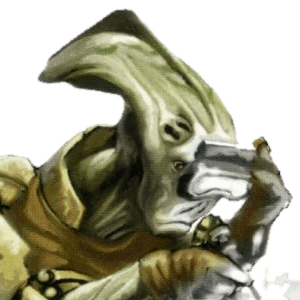
\includegraphics[width=\linewidth]{_img/pnjs/vyna-anen.png}
\textbf{Race:} Sluissi

\subsubsection{Background}

Vyna Anen est l’un des agents de liaison entre Industrial Automaton et l’Empire. Officiellement employé par IA comme secrétaire au service des "Projets Spéciaux". 

Vyna est un homme pragmatique qui fait ce que l’Empire lui demande sans poser de questions, sans scrupules ni états d’âme. C’est un fin négociateur entièrement voué à l’Empire.

\subsubsection{Traits}

\begin{itemtable}[ c c c c c ]
    \textbf{Agi} & \textbf{Int} & \textbf{\^Ame} & \textbf{For} & \textbf{Vig} \\
    d6           & d10          & d6             & d4           & d6
\end{itemtable}
\begin{itemtable}[ l X ]
    \textbf{Allure}      & 6 \\
    \textbf{Compétences} & Intimidation d6, Persuasion d12, Réseaux d6
\end{itemtable}

\subsubsection{Défense}
\begin{itemtable}[ c c ]
    \textbf{Parade}     & \textbf{Résistance} \\
    2                   & 5 
\end{itemtable} 

\clearpage
\onecolumn
\label{sec:r4-3d}
\begin{tikzpicture}[overlay, anchor=north]
    \node at (9,2) {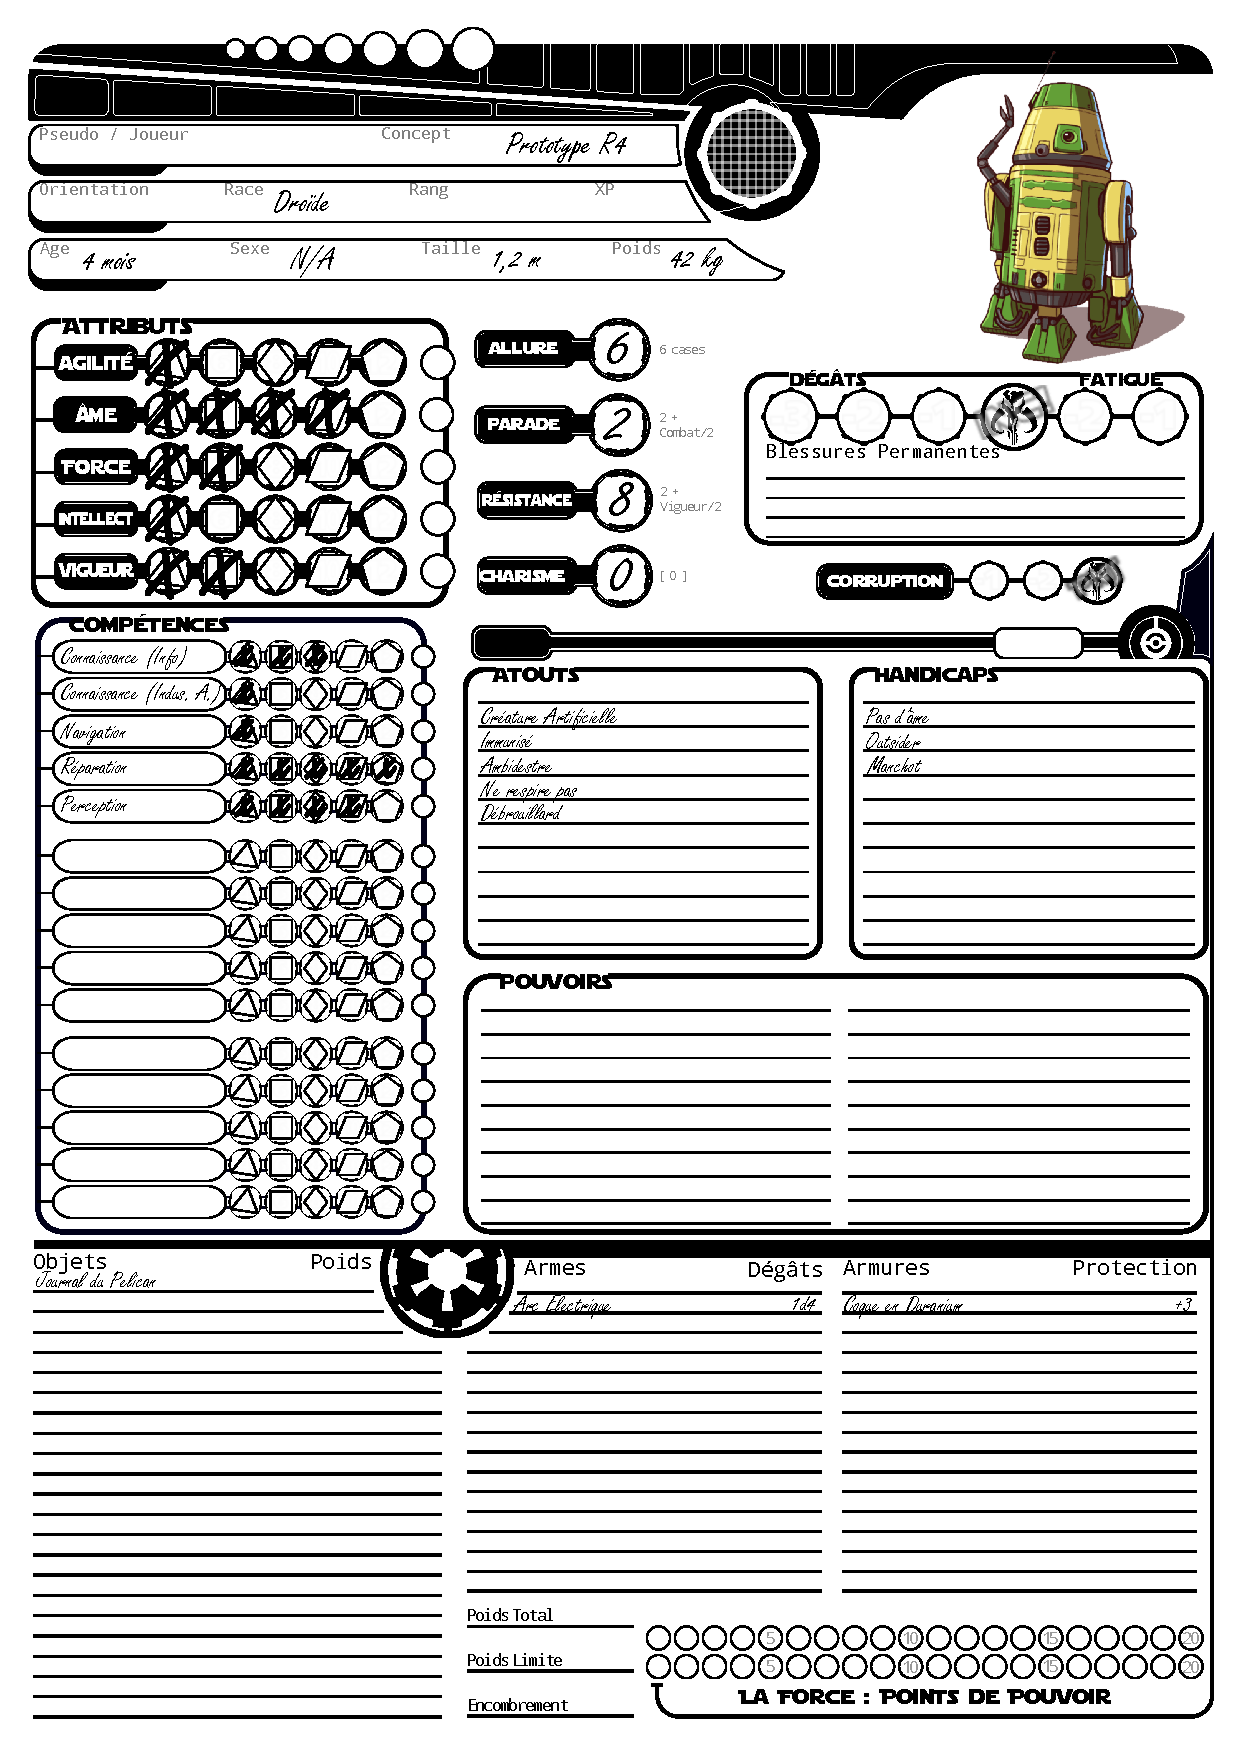
\includegraphics[height=\paperheight]{tex/R4-3D.pdf}};
\end{tikzpicture}

\twocolumn 
\clearpage
\subsection{Tinon Dystra} \label{sec:tinon-dystra}
\begin{figure}[h!]
    \centering
    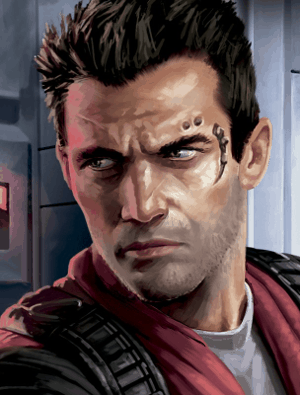
\includegraphics[height=250pt]{_img/pnjs/tinon-dystra.png}
\end{figure}

\subsubsection{Background}
Ce personnage est mort quand débute le scénario mais il garde son importance car il est le lien entre les joueurs et l'alliance Rebelle.

Tinon est un membre de l'alliance rebelle envoyé en mission d'infiltration sur un vaisson de Industrial Automaton (Le \nameref{sec:pelican}) afin de découvrir ce qu'il s'y trame. Mais sa mission à mal tourné et il n'a plus donné aucune nouvelle. 

En fait il s'est infiltré à bord du Pelican alors que la maladie des \nameref{sec:rakghoul} était en train de s'y répandre. A bord du Pelican il s'est fait infecté et s'est transformé en Rakghoul lui-même. Son vaisseau, le \nameref{sec:nimbus} est resté à quai sur le Pelican.

Tinon avait une relation avec \nameref{sec:lindi-dangon}.

\newpage
\subsection{Lindi Dangon} \label{sec:lindi-dangon}
\begin{figure}[h!]
    \centering
    
\includegraphics[height=250pt]{_img/pnjs/lindi-dangon.png}
\end{figure}
\subsubsection{Background}
Lindi Dangon commande l'une des cellule de résistance dans la zone de Taris. C'est elle qui a ordonné la mission durant laquelle \nameref{sec:tinon-dystra} à disparut. Elle se sent d'autant plus coupable que Tinon était son amant et depuis sa disparition elle n'a de sesse de la retrouver. Elle garde espoir tant qu'elle n'a pas de preuve de sa mort.

\subsubsection{Traits}

\begin{itemtable}[ c c c c c ]
    \textbf{Agi} & \textbf{Int} & \textbf{\^Ame} & \textbf{For} & \textbf{Vig} \\
    d6           & d10          & d8             & d4           & d4           
\end{itemtable}
\begin{itemtable}[ l X ]
    \textbf{Allure}      & 6 \\
    \textbf{Compétences} & Intimidation d8, Persuasion d8, Réseaux d10, Tir d10, Combat d4 \\
    \textdb{Atouts}      & Commandement
\end{itemtable}

\subsubsection{Défense}
\begin{itemtable}[ c c ]
    \textbf{Parade}     & \textbf{Résistance} \\
    5                   & 3 
\end{itemtable}

\newpage
\subsection{Garan Keggle}  \label{sec:garan-keggle}
\begin{figure}[h!]
    \centering
    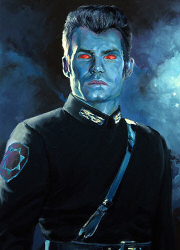
\includegraphics[height=200pt]{_img/pnjs/garan-keggle.png}
\end{figure}
\vspace{-1\baselineskip}
\subsubsection{Background}
Officier supérieur dans l'armée de l'empire, Garan Keggle dirige les recherches d'artéfacts Sith pour le compte de l'empereur et son second Dark Vador. Suite à des informations sur le Talisman de Muur, il a dépéché un vaisseau de l'Insdustrial Automaton pour récupérer l'artéfact sur Taris sous couvert de projet scientifique.

Son contact chez IA est \nameref{sec:vyna-anen}, de manière générale Garan n'a que très peu de contact avec ses sous-traitant pour éviter que les ennuis remontent jsuqu'à l'empire. 

Garan est un home déterminé et sans pitié, initié au coté obscur de la Force, il attend la première occasion pour se débarrasser de ses rivaux et pouvoir prétendre au plus vite à la place d'apprenti et plus tard de seigneur Sith.

\subsubsection{Traits}
\begin{itemtable}[ c c c c c ]
    \textbf{Agi} & \textbf{Int} & \textbf{\^Ame} & \textbf{For} & \textbf{Vig} \\
    d6           & d10          & d10            & d6           & d8           
\end{itemtable}
\begin{itemtable}[ l X ]
    \textbf{Allure}      & 6 \\
    \textbf{Compétences} & Intimidation d10, Tir d10, Combat d8, Maitrise Force d8, Perception d6 \\
    \textdb{Atouts}      & Commandement, Grande aura de commandement
\end{itemtable}

\subsubsection{Défense}
\begin{itemtable}[ c c ]
    \textbf{Parade}     & \textbf{Résistance} \\
    6                   & 6 
\end{itemtable}

\newpage
\subsection{Gil Harend}  \label{sec:gil-harend}
\begin{figure}[h!]
    \centering
    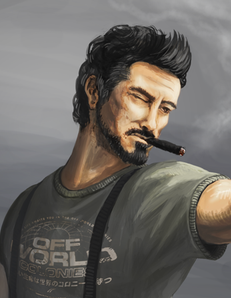
\includegraphics[height=200pt]{_img/pnjs/gil-harend.png}
\end{figure}
\subsubsection{Background}
Double background selon la voie choisie.

Gil Harend est un père qui essai tant bien que mal d'élever sa fille de 16 ans, Abygaelle, dans les bas fonds de Taris. Depuis la disparition se sa femme Karie, la vie est très difficile. De plus les contrebandiers font régulièrement des razzia dans leur village pour kidnapper les jeunes filles et les revendre comme esclaves. Il y a deux jours, c'est Abygaelle qui a été enlevée. Gil fera tout pour la retrouver.\\

Gil Harend est un contrebandier qui opère dans les bas fonds de Taris. Avec ses 3 accolytes Gil fait des petits boulots plus ou moins légaux mais ce qui rapporte le plus c'est la revente de jeunes esclaves. Il y a 2 jours, lui est son équipe on kidnappés une jeune fille de 16 ans dans un village des bas fonds.

\subsubsection{Traits}
\begin{itemtable}[ c c c c c ]
    \textbf{Agi} & \textbf{Int} & \textbf{\^Ame} & \textbf{For} & \textbf{Vig} \\
    d4           & d8           & d4             & d8           & d8           
\end{itemtable}
\begin{itemtable}[ l X ]
    \textbf{Allure}      & 6 \\
    \textbf{Compétences} & Tir d6, Combat d4, Persuasion d6
\end{itemtable}

\subsubsection{Défense}
\begin{itemtable}[ c c ]
    \textbf{Parade}     & \textbf{Résistance} \\
    4                   & 6 
\end{itemtable}

\newpage
\subsection{Pulsipher} \label{sec:pulsipher}
\begin{figure}[h!]
    \centering
    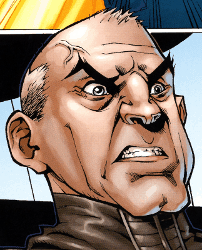
\includegraphics[height=200pt]{_img/pnjs/pulsipher.png}
\end{figure}

\subsubsection{Background}
Pulsipher est un Mandalorien qui vécut plus de 3000 ans avant l'avènement de l'empire. Scientifique Néo-Croisé, il s'intéressait à la Force et tout ce qui s'y rattache. Il était persuadé que le secret de la Force lui permettrait de mettre fin à la guerre. 

C'est lui qui découvrit dans les bas-fonds de Taris et qui le ramena sur Jebble.

\subsubsection{Traits}
\begin{itemtable}[ c c c c c ]
    \textbf{Agi} & \textbf{Int} & \textbf{\^Ame} & \textbf{For} & \textbf{Vig} \\
    d4           & d12          & d4             & d8           & d6           
\end{itemtable}
\begin{itemtable}[ l X ]
    \textbf{Allure}      & 6 \\
    \textbf{Compétences} & Tir d8, Combat d8, Persuasion d6, Connaissance d12
\end{itemtable}

\subsubsection{Défense}
\begin{itemtable}[ c c ]
    \textbf{Parade}     & \textbf{Résistance} \\
    6                   & 8 
\end{itemtable}

\newpage
\subsection{Lucy} \label{sec:lucy-pher}
\begin{figure}[h!]
    \centering
    
\includegraphics[height=200pt]{_img/pnjs/lucy.png}
\end{figure}

\subsubsection{Background}
Lucy est une IA particulièrement avancée (même pour la période du JdR). Mise au point par Pulsipher lui-même a partir d’un modèle de base, elle est la gardienne du Laboratoire et de tout se qu’il renferme. \'A l’époque où le labo était en activité, Lucy prenait en charge la plupart des caculs à effectuer sur l’ensemble des recherches. Elle était même capable d’anticiper certains résultats et d’ajuster les expériences de manière proactive.

Elle possède un plein accès au laboratoire, et par un réseau de caméra elle peut tout y voir.

\subsubsection{Traits}
\begin{itemtable}[ c c c c c ]
    \textbf{Agi} & \textbf{Int} & \textbf{\^Ame} & \textbf{For} & \textbf{Vig} \\
    d0           & d12+4        & d0             & d0           & d8           
\end{itemtable}
\begin{itemtable}[ l X ]
    \textbf{Allure}      & 0 \\
    \textbf{Compétences} & Tir d10, Combat d0, Persuasion d10, Connaissance d12
\end{itemtable}

\subsubsection{Défense}
\begin{itemtable}[ c c ]
    \textbf{Parade}     & \textbf{Résistance} \\
    0                   & 6 
\end{itemtable}

\newpage
\subsection{Céleste Morne*} \label{sec:celeste-morne}
\begin{figure}[h!]
    \centering
    
\includegraphics[height=200pt]{_img/pnjs/celeste-morne.png}
\end{figure}

\subsubsection{Background}
Issue d’une famille de Jedi établie à Ossus, elle perdie tout ce qu’elle avait quand les Siths dévastèrent la planète durant la grande guerre des Siths. Sous la tutelle de Krynda Draay elle fut formée aux arts Jedi et, après une formation d’Ombre Jedi, elle fut recruté par le Covenant.

C’est en tant qu’Ombre du Covenant qu’elle partie en mission pour retrouver le Talisman de Muur et qu’elle croisa la route de \nameref{sec:pulsipher}. Lors de sa tentative pour sauver ce dernier et pour récupérer l’artéfact, celui-ci, attiré par les pouvoir de Céleste pris possession de son corps. Céleste parveint à le maitriser juste assez longtemps pour que Zayne Carrick, son apprenti l’enferme dans l’\nameref{sec:oubliette-de-dreypa}.

\subsubsection{Traits}
\begin{itemtable}[ c c c c c ]
    \textbf{Agi} & \textbf{Int} & \textbf{\^Ame} & \textbf{For} & \textbf{Vig} \\
    d10          & d8           & d10            & d6           & d8           
\end{itemtable}
\begin{itemtable}[ l X ]
    \textbf{Allure}      & 0 \\
    \textbf{Compétences} & Tir d6, Combat d12, Persuasion d10, Maitrise de la force d12
\end{itemtable}

\subsubsection{Défense}
\begin{itemtable}[ c c ]
    \textbf{Parade}     & \textbf{Résistance} \\
    8                   & 6 
\end{itemtable}

\newpage
\subsection{Fane Peturri} \label{sec:fane-peturri}
\begin{figure}[h!]
    \centering
    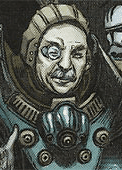
\includegraphics[height=200pt]{_img/pnjs/fane-peturri.png}
\end{figure}

\subsubsection{Background}
Fane Peturri était un historien qui vécut durant les derniers décennies de la République et au tout début de l'Empire. Il semble qu'il était également un vieil ami de Palpatine et un des rares à savoir que celui-ci était un Seigneur Sith, ce qui fit qu'il eut des liens étroits avec l'Empire dès sa proclamation.

\subsubsection{Traits}
\begin{itemtable}[ c c c c c ]
    \textbf{Agi} & \textbf{Int} & \textbf{\^Ame} & \textbf{For} & \textbf{Vig} \\
    d6           & d10          & d4             & d6           & d8           
\end{itemtable}
\begin{itemtable}[ l X ]
    \textbf{Allure}      & 6 \\
    \textbf{Compétences} & Tir d4, Réseau d10, Connaissance (Empire) d10, Connaissance (Sith) d10
\end{itemtable}

\subsubsection{Défense}
\begin{itemtable}[ c c ]
    \textbf{Parade}     & \textbf{Résistance} \\
    4                   & 6 
\end{itemtable}

\newpage
\subsection{Schurk-Heren}\label{sec:schurk-heren}
\begin{figure}[h!]
    \centering
    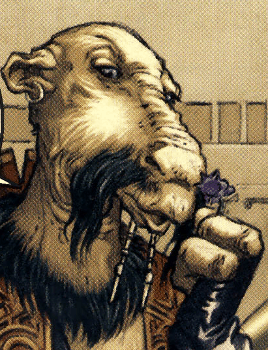
\includegraphics[height=200pt]{_img/pnjs/schurk-heren.png}
\end{figure}

\newpage
\subsection{Dass Jennir} \label{sec:dass-jennir}
\begin{figure}[h!]
    \centering
    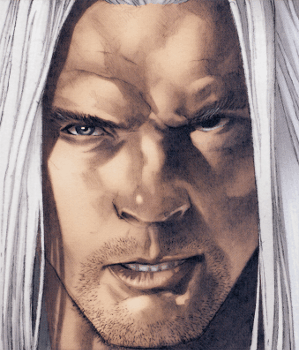
\includegraphics[height=200pt]{_img/pnjs/dass-jennir.png}
\end{figure}

\newpage
\subsection{Queen Jool} \label{sec:queen-jool}
\begin{figure}[h!]
    \centering
    
\includegraphics[height=200pt]{_img/pnjs/queen-jool.png}
\end{figure}
	\section{Bestiaire}\label{sec:bestiaire}

\subsection{Rakghoul}
\label{sec:rakghoul}
\noindent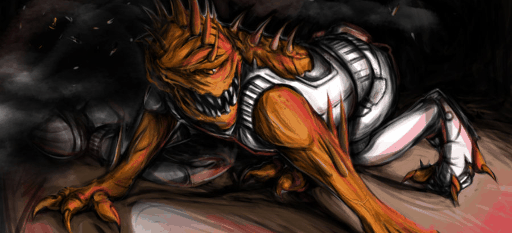
\includegraphics[width=\linewidth]{_img/bestiary/rakghoul.png}

\paragraph{Background}
Les Rakghouls sont une espèce issue d’une maladie créée par le seigneur Sith Karness Muur. Les individus atteint par cette maladie deviennent des monstres incapables de penser par eux-mêmes. Karness peut les contrôler grâce à son talisman (Le Talisman de Muur).

La maladie se transmet par une griffure ou une morsure mais cela ne fonctionne pas avec les êtres sensibles à la Force. Karness a créé ce virus à partir du coté Obscur de la Force ce qui explique une forte présence obscure près de ces monstres.

Karness a créé plusieurs versions du virus car les premiers Rakghouls ne répondaient pas bien au contrôle de Karness. Les nouveaux sont plus réceptifs et plus fort.

Quand le Talisman de Muur a été perdu dans les bas fonds de Taris, on a peu constaté que les créatures, suite à une exposition prologée au Talisman finissaient par se transformer en Rakghouls. Mais les Rakghouls transformé de cette façon sont bestiaux, stupides et sans âme. Ils attaquent tout ce qui bouge. Ces créatures ne fonctionnent qu’à l’instinct.

\paragraph{Traits}

\begin{itemtable}[ c c c c c ]
    \textbf{Agi} & \textbf{Int} & \textbf{\^Ame} & \textbf{For} & \textbf{Vig} \\
    d8           & d6           & d6             & d8           & d8
\end{itemtable}
\begin{itemtable}[ l X ]
    \textbf{Allure}      & 6 \\
    ~                    & Vision Nocturne \\
    ~                    & Marche sur les murs \\
    \textbf{Compétences} & Combat d8, Discrétion d6
\end{itemtable}

\paragraph{Attaque / Défense}
\begin{itemtable}[ c c ]
    \textbf{Parade}     & \textbf{Résistance} \\
    6                   & 6 
\end{itemtable}

\begin{itemtable}[ X c c ]
    ~       & \textbf{Combat}   & \textbf{Dégats} \\
    Griffes & d8                & 1d6 
\end{itemtable}

\newpage
\subsection{Rakghoul Amblyope}
\label{sec:rakghoul-amblyope}
\noindent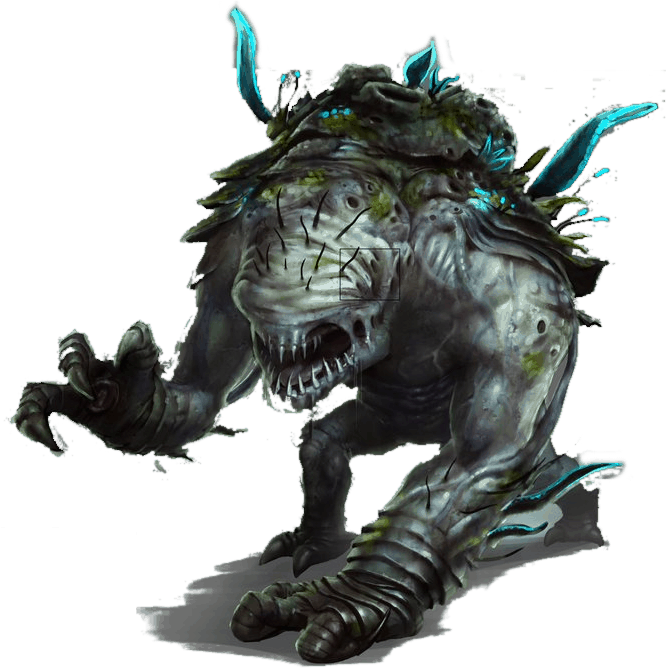
\includegraphics[height=200pt]{_img/bestiary/rakghoul-amblyope.png}

\paragraph{Background}
Version stéroïdée des Rakghouls standard, Amblyope est notre petit boss de niveau.

Quand les Rakghouls sont livrés à eux-mêmes et qu’ils laissent libre cours à leurs plus bas instincts, il arrive qu’un Rakghoul plus fort que les autres s’en prenne à ces petits camarades et les dévore sans scrupules. Cet afflux de Force Obscure peut le faire muter et le Rakghoul devient une espèce de gros monstre de 3m de haut, complètement aveugle mais attiré par les émanations de Force, il attaque machinalement les adversaires les plus sensibles à la Force. 

\paragraph{Traits}

\begin{itemtable}[ c c c c c ]
    \textbf{Agi} & \textbf{Int} & \textbf{\^Ame} & \textbf{For} & \textbf{Vig} \\
    d4           & d6           & d6             & d12+2        & d10
\end{itemtable}
\begin{itemtable}[ l X ]
    \textbf{Allure}      & 5 \\
    \textbf{Taille}      & +5 \\
    ~                    & Vision de Force \\
    ~                    & \'Enorme (+2 pour les jets d’attaque adverses)\\
    \textbf{Compétences} & Combat d10
\end{itemtable}

\paragraph{Défense / Attaque}
\begin{itemtable}[ c c ]
    \textbf{Parade}     & \textbf{Résistance} \\
    5                   & 12 
\end{itemtable}

\begin{itemtable}[ X c c ]
    ~           & \textbf{Combat}   & \textbf{Dégats} \\
    Mains nues  & d10               & d12+2 
\end{itemtable}

\clearpage

\subsection{Contrebandier (Taris)} \label{sec:taris-contrebandier}
\begin{figure}[h!]
    \centering
    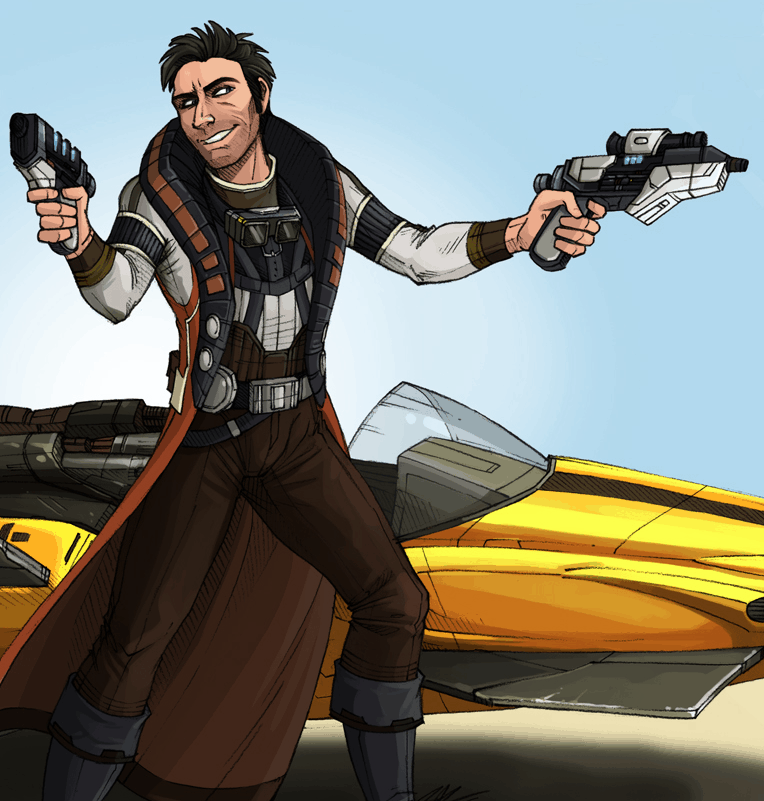
\includegraphics[height=200pt]{_img/bestiary/contrebandier.png}
\end{figure}
\paragraph{Background}
Les bas-fonds de Taris grouillent de toutes sortes de malfrats. C’est un des coins favoris de contrebandiers qui peuvent y kidnapper de jeunes enfants en toute impunité. Personne ne viendra se plaindre de la disparition d’une vermine de plus dans les bas fond.

Ce ne sont en général que des débutants attiré par la facilité. Seul ils ne représentent pas un grand danger, mais ils se promènent souvent en groupe.

\paragraph{Traits}

\begin{itemtable}[ c c c c c ]
    \textbf{Agi} & \textbf{Int} & \textbf{\^Ame} & \textbf{For} & \textbf{Vig} \\
    d6           & d6           & d4             & d8           & d8
\end{itemtable}
\begin{itemtable}[ l X ]
    \textbf{Allure}      & 6 \\
    \textbf{Compétences} & Combat d8, Tir d10
\end{itemtable}

\paragraph{Défense}
\begin{itemtable}[ c c ]
    \textbf{Parade}     & \textbf{Résistance} \\
    5                   & 6 (+1)
\end{itemtable}

\paragraph{Attaque}
\begin{itemtable}[ X c c ]
    ~           & \textbf{Combat}   & \textbf{Dégats} \\
    Blaster     & -                 & 2d6+1
\end{itemtable}


\newpage

\subsection{Storm Trooper} \label{sec:storm-trooper}
\begin{figure}[h!]
    \centering
    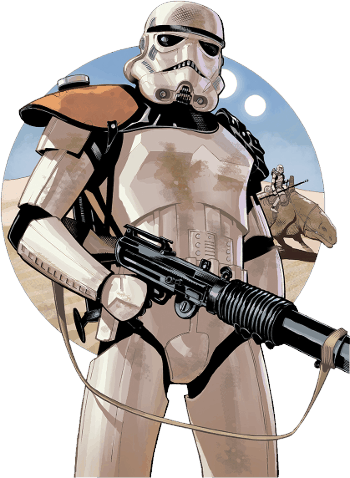
\includegraphics[height=200pt]{_img/bestiary/stormtrooper.png}
\end{figure}
\paragraph{Background}
Soldats dévoué de l’empire. Certain sont des clones restant de la guerre des clones d’autres non. Ils sont entrainés au combat, équipé d’une bonne armure et armé de Fusil Blaster efficaces.

\paragraph{Traits}

\begin{itemtable}[ c c c c c ]
    \textbf{Agi} & \textbf{Int} & \textbf{\^Ame} & \textbf{For} & \textbf{Vig} \\
    d4           & d6           & d4             & d8           & d8
\end{itemtable}
\begin{itemtable}[ l X ]
    \textbf{Allure}      & 6 \\
    \textbf{Compétences} & Combat d10, Tir d10
\end{itemtable}

\paragraph{Défense}
\begin{itemtable}[ c c ]
    \textbf{Parade}     & \textbf{Résistance} \\
    7                   & 6 (+4)
\end{itemtable}

\paragraph{Attaque}
\begin{itemtable}[ X c c ]
    ~              & \textbf{Combat}   & \textbf{Dégats} \\
    Fusil Blaster  & -                 & 2d8 (3)
\end{itemtable}


\newpage
\subsection{Wampa} \label{sec:wampa}
\begin{figure}[h!]
    \centering
    
\includegraphics[height=200pt]{_img/bestiary/wampa.png}
\end{figure}

\paragraph{Background}
Créature capable de supporter les plus froides températures, le Wampa est un féroce prédateur agissant surtout la nuit. Bien que sa planète d’origine soit Hoth, on retrouve des Wampas sur quelques autres mondes, mais leur férocité les rend difficiles à exporter, et on trouve peu de candidats assez fous pour tenter l’expérience. 

\paragraph{Traits}

\begin{itemtable}[ c c c c c ]
    \textbf{Agi} & \textbf{Int} & \textbf{\^Ame} & \textbf{For} & \textbf{Vig} \\
    d8           & d6           & d6             & d8           & d8
\end{itemtable}
\begin{itemtable}[ l X ]
    \textbf{Allure}      & 6 \\
    ~                    & Vision Nocturne \\
    ~                    & Marche sur les murs \\
    \textbf{Compétences} & Combat d8, Discrétion d6
\end{itemtable}

\paragraph{Attaque / Défense}
\begin{itemtable}[ c c ]
    \textbf{Parade}     & \textbf{Résistance} \\
    6                   & 6 
\end{itemtable}

\begin{itemtable}[ X c c ]
    ~       & \textbf{Combat}   & \textbf{Dégats} \\
    Griffes & d8                & 1d6 
\end{itemtable}

\newpage

\subsection{Cybercleps} \label{sec:cybercleps}
\begin{figure}[h!]
    \centering
    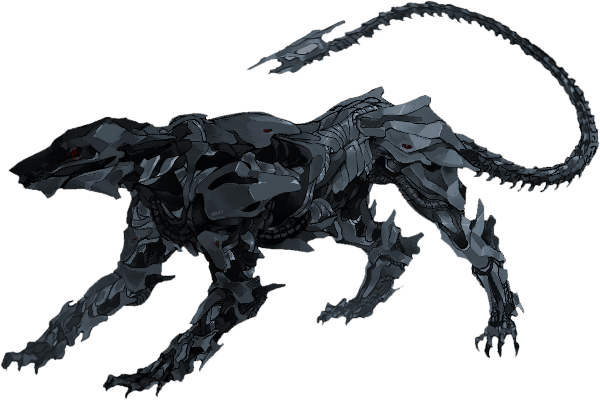
\includegraphics[width=\linewidth]{_img/bestiary/cybercleps.png}
\end{figure}
\paragraph{Background}
Les Cybercleps sont des créatures artificielles conçues pour tenir éloigné les curieux de certaines zones. Ce sont des drônes capable d’une complète autonomie mais leur efficacité est bien meilleure quand elles sont contrôllé par une IA centrale. 

Adaptées au gardiennage de batiments de à la sécurité des villas, leur conception ne les prédestine pas à devenir des animaux de compagnie, même avec la programmation adéquate !

Lorsqu’ils sont commandé par un central, leur programmation les rend particulièrement efficace. Ils deviennent capable d’attaquer en groupe et de se concentrer sur les proies plus faible. Ils sont capable de stratégies de combat pour venir à bout de groupe plus nombreux qu’eux.

Les Cybercleps restent combatif même blessé grièvement, tant que le processeur principal présent dans leur tête n’est pas détruit.
\paragraph{Traits}

\begin{itemtable}[ c c c c c ]
    \textbf{Agi} & \textbf{Int} & \textbf{\^Ame} & \textbf{For} & \textbf{Vig} \\
    d8           & d4           & d4             & d8           & d8
\end{itemtable}
\begin{itemtable}[ l X ]
    \textbf{Allure}      & 7 \\
    \textbf{Compétences} & Combat d10 \\
    \textbf{Atouts}      & Grande esquive \par Créature artificielle
\end{itemtable}

\paragraph{Défense / Attaque}
\begin{itemtable}[ c c ]
    \textbf{Parade}     & \textbf{Résistance} \\
    8                   & 6
\end{itemtable}

\begin{itemtable}[ X c c ]
    ~              & \textbf{Combat}   & \textbf{Dégats} \\
    Griffe         & -                 & 1d8 (2)         \\
    Crocs          & -                 & 2d6 (1)
\end{itemtable}

\subsection{Corvette class Raider} \label{sec:empire-corvette}
\begin{figure}[h!]
    \centering
    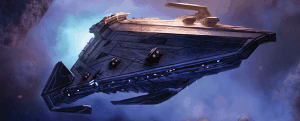
\includegraphics[width=\linewidth]{_img/bestiary/raider-corvette.png}
\end{figure}

\paragraph{Background}
La corvette de classe Raider est un vaisseau anti-chasseurs à la fois léger et moderne. C’est un vaisseau capable à la fois de déployer des \nameref{sec:tie-fighter} et de les défendre face aux chasseurs ennemis. 

Longue de 150 mètres, le classe Raider est donc un vaisseau robuste en forme de dague et dont la passerelle située à la poupe - pour des raisons évidentes d’échelle et de sécurité - dépasse à peine de sa carlingue. 

\paragraph{Traits}

\begin{itemtable}[ c c c c ]
    \textbf{Size} & \textbf{Acc/VMax} & \textbf{Climb} & \textbf{Rés.} \\
    150m          & 35/400            & 1              & 45 (10)       
\end{itemtable}

\paragraph{Défense / Attaque}
\begin{itemtable}[ X c c ]
    \textbf{Arme}     & \textbf{Portée} & \textbf{Dégats}       \\
    Canon Lourd (x6)  & 600             & 4d10                  \\
    Canon Ionique*    & 600             & 1d10 (immobilisant)
\end{itemtable}
* Un tir de Canon Ionique, s’il touche, immobilise la cible. Tout ce qui est électrique à bord du vaisseau ne fonctionne plus (armes, bouclier, propulsion, \ldots). Une réparation est nécessaire pour repartir. La difficulté de la réparation est de -4, -8 si l’attaque a touché avec une relance.

\newpage
\subsection{Chasseur TIE} \label{sec:tie-fighter}
\begin{figure}[h!]
    \centering
    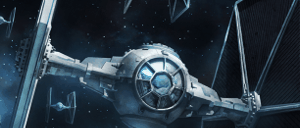
\includegraphics[width=\linewidth]{_img/bestiary/tie-fighter.png}
\end{figure}

\paragraph{Background}
Les TIEs possèdent des caractéristiques communes : un système de propulsion basé sur un double moteur ionique (d’où le nom de T.I.E. : Twin Ion Engine, ou double moteur ionique, une alimentation basée sur des panneaux solaires, et généralement un équipement minimaliste, tant au niveau des systèmes de survie que de l’hyperpropulsion. Tout équipement «~superflu~» est supprimée, de manière à obtenir un appareil peu onéreux.

\begin{itemtable}[ c c c c ]
    \textbf{Size} & \textbf{Acc/VMax} & \textbf{Climb} & \textbf{Rés.} \\
    6m            & 50/700            & 1              & 20 (5)       
\end{itemtable}

\paragraph{Défense / Attaque}
\begin{itemtable}[ X c c ]
    \textbf{Arme}      & \textbf{Portée} & \textbf{Dégats}       \\
    Double Canon Léger & 500             & 2d10                  \\
\end{itemtable}

	\onecolumn
	\nocite{*}
	\printbibliography
\end{document}